\documentclass[twoside]{book}
\usepackage[top=0.9in, bottom=0.9in,left=0.9in, right=0.9in, paperwidth=6in, paperheight=9in]{geometry}
\usepackage{puzzles}

\begin{document}
\title{Математические головоломки}
\author{Питер Винклер}
\date{}
\maketitle

\chapter*{Интуиция}
 

\epigraph{Когда напряженная умственная работа сменяется периодами отдыха, интуиция словно берет верх, и порождает кристально ясные откровения, привносящие в процесс научного исследования неповторимое удовольствие и наслаждение.}{Фритьоф Капра, физик}

Эта глава предназначена для разминки и содержит задачи, не относящиеся к какой-либо специфической теме или технике.
Однако, как часто бывает в таких случаях, некоторые ключевые идеи могут помочь вам в дальнейшем.
 Вот для начала одна из подобных задач:

\subsection*{Монеты в ряд} %(COINS IN A ROW)

На столе выложен ряд из пятидесяти монет различного достоинства.
Алиса берет монету с одного конца и кладет себе в карман, затем Боб выбирает монету с одного из концов, и так они продолжают по очереди, пока Боб не забирает последнюю монету.

Докажите, что Алиса может вести игру таким образом, что, по крайней мере, сможет набрать денег не меньше, чем Боб.

\medskip

Попробуйте сыграть в эту игру сами, для начала с несколькими монетами (или случайными числами), начните с 4 или 6 вместо 50.
Совсем неочевидно, как играть оптимально, не так ли?
Но, может Алисе и не нужна оптимальная стратегия? 

Сейчас у Вас подходящий момент установить себе правило --- пытаться решить задачу до того, как вы продолжите чтение.

\paragraph{Решение:}
Пронумеруем все монеты от 1 до 50 и заметим, что, независимо от того, как ходит Боб, Алиса может забрать все чётные или, если она предпочитает, все нечётные монеты.
Один из этих выборов должен, по крайней мере, не уступать другому.
\heart

Эту задачу я узнал от Эхуда Фридгута;
говорят, что её давали при приеме на работу в одной израильской ИТ компании.
Вообщем-то у Алисы есть более оптимальные стратегии, чем выбор всех чётных или нечётных монет.
Заметим, однако, что если у нас 51 монета вместо 50, то Боб (игрок, который ходит вторым) обычно обладает преимуществом, несмотря на меньшее, чем у Алисы, количество собранных монет.
Кажется парадоксальным, что чётность числа монет имеет такой огромный эффект на результат игры, при том, что монеты берутся только с концов.

\medskip

Ну что ж, попробуйте теперь сами.
Мы начнем с двух менее математических задач, а затем перейдем к вещам посерьезнее.
И~пусть ваше воображение укажет вам верный путь!

\subsection*{Два Биксби} %(THE BIXBY BOYS)

Это был первый день школы и Миссис Фелдман, войдя в класс, увидела сидящих за первой партой двух абсолютно одинаковых учеников, Дональда и Рональда Биксби.

--- Вы двойняшки, не так ли? --- спросила она.

--- Нет, --- ответили они хором.

Миссис Фелдман проверила записи в журнале и убедилась, что у мальчиков одни и те же родители и родились они в один и тот же день.
Как такое может быть?

\subsection*{Свет на чердаке} %(THE ATTIC LAMP SWITCH)

На первом этаже дома находится панель с тремя выключателями, один из них включает свет на чердаке --- но который? 
Ваша задача --- совершить некие действия с выключателями и после одного похода на чердак определить, какой выключатель подключен к чердачной лампочке.

\subsection*{Бензиновый кризис} %(GASOLINE CRISIS)

Представьте, что у нас кризис --- не хватает бензина.
Заправочные станции, расположенные на большой кольцевой дороге, обладают все вместе количеством бензина, достаточным только для одного проезда по кольцу.
Докажите, что, отправившись с правильной автозаправки с пустым баком, вы сможете проехать по всей кольцевой дороге.

\subsection*{Бикфордовы шнуры} %(USES OF FUSES)

У вас имеются два бикфордовых шнура (т.~е. два куска огнепроводного шнура), каждый из них сгорает ровно за одну минуту, но горение неравномерно по длине шнура.
Можно ли при помощи этих двух бикфордовых шнуров отмерить 45 секунд?

\subsection*{Целые числа и прямоугольники} %(INTEGERS AND RECTANGLES)

Большой прямоугольник на плоскости разбит на малые прямоугольники, у каждого из которых либо высота, либо основание, либо оба --- целое число. 
Докажите, что большой прямоугольник также обладает этим свойством.

\begin{figure}[h!]
\centering
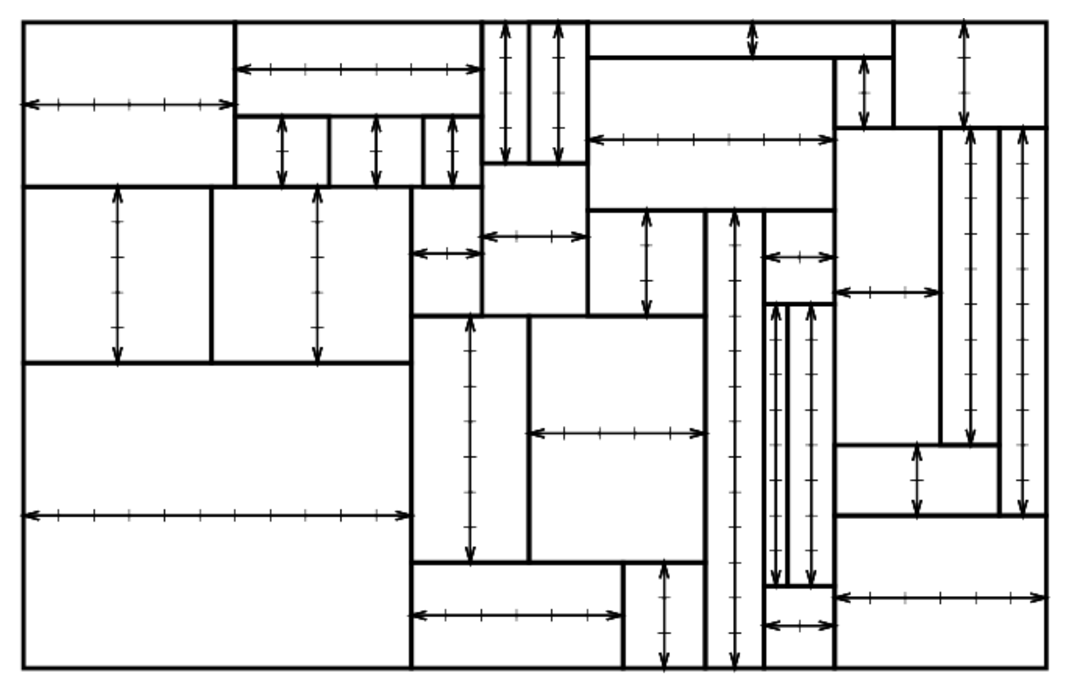
\includegraphics[scale=0.6]{Figs/Insight/rect}
\end{figure}

\subsection*{Весы и гири} %(TIPPING THE SCALES)

На столе у учителя стоят чашечные весы, правая чашка весов перевешивает.
На весах стоят гири не обязательно одного веса, на каждой из которых написаны фамилии одного \emph{или нескольких} учеников.
Ученик, входя в класс, переставляет на другую чашку весов каждую гирю, на которой написана его фамилия.
Докажите, что можно впустить в класс таких учеников, чтобы в результате перевесила левая чашка весов.

\subsection*{Часы на столе} %(WATCHERS ON THE TABLE)

На столе лежат пятьдесят точных ручных часов.
Докажите, что существует момент времени, когда сумма расстояний от центра стола до кончиков минутных стрелок больше, чем сумма расстояний от центра стола до центров часов.

\subsection*{Путь по шахматной доске} %(PATH ON CHESSBOARD)

Алиса начинает игру и ставит фишку в угол шахматной доски размером $n{\times}n$ клеток.
Боб передвигает фишку на соседнее поле, имеющее общую сторону с тем, на котором стоит фишка.
Второй раз ходить на поле, где уже побывала фишка, нельзя. 
Алиса и Боб ходят по очереди.
Проигрывает тот, кому некуда ходить.

При каких $n$ у Алисы есть выигрышная стратегия? 
При каких $n$ она выигрывает, если ее первый ход не на угловое поле, а на соседнее с ним?

\subsection*{Степень в степени} %(EXPONENT UPON EXPONENT)

На экзамене по математике для старших классов Американской школы 1960-х годов 
был следующий вопрос:
Если 
$$x^{x^{x^{{\cdot}^{\cdot^{\cdot}}}}}=2$$
Чему равен $x$? 
Предполагаемое решение основывается на том, что степень «нижнего» $x$ равна всему выражению, таким образом $x^2\z=2$ и $x=\sqrt{2}$.
Но один ученик заметил, что если бы в задаче спрашивалось решение
$$x^{x^{x^{{\cdot}^{\cdot^{\cdot}}}}}=4$$
то он бы получил тот же ответ: $x=\sqrt[4]{4}=\sqrt{2}$

Хмм...
Чему же тогда равно ${\sqrt{2}}^{{\sqrt{2}}^{{\sqrt{2}}^{{\cdot}^{\cdot^{\cdot}}}}}$? 
Можете это доказать?

\subsection*{Солдаты в поле} %(SOLDIERS IN THE FIELD)

Нечётное число солдат расположилось на поле таким образом, что все попарные расстояния между ними (между каждой парой солдат) различны.
При этом каждый солдат должен присматривать за ближайшим к нему другим солдатом.

Докажите, что существует хотя бы один солдат, за которым никто не присматривает.

\subsection*{Отрезки и расстояния} %(INTERVALS AND DISTANCES)

Пусть множество $S$ состоит из $k$ непересекающихся отрезков, лежащих в единичном отрезке $[0,1]$.
Предположим, что $S$ обладает следующим свойством: для любого вещественного числа $d$ из отрезка $[0,1]$, в множестве $S$ существуют две точки на расстоянии $d$ друг от друга.
Докажите, что сумма длин отрезков $S$ не меньше $1/k$.

 
\subsection*{Собрать 15} %(SUMMING TO 15)

Алиса и Боб по очереди выбирают число из $1, 2,\dots,9$, без повторов.
Выигрывает тот, кто первый наберет три числа, дающие в сумме 15.
Имеется ли у Алисы (она ходит первая)
выигрышная стратегия?

%ё
\section*{Решения и комментарии}

\subsubsection*{Два Биксби} % (THE BIXBY BOYS)

Классическая головоломка.
Конечно же, это были тройняшки.
Третий близнец (Арнольд?) учился в другом классе.

\subsubsection*{Свет на чердаке} % (THE ATTIC LAMP SWITCH)

Эта задача пронеслась по миру, как эпидемия гриппа, где-то лет десять тому назад; я не знаю её источника.

Действительно, невозможно определить, какой выключатель подключён к лампочке на чердаке, если всё, что у вас имеется --- это один бит информации, полученный от вашего похода на чердак.
Однако, вы можете добыть больше сведений, если используете ваши руки!
Включите выключатели 1 и 2, подождите несколько минут, затем выключите второй выключатель и идите на чердак.
Если лампочка не горит, но горячая, значит, второй выключатель это то, что мы ищем.
\heart

Если вы не можете дотянуться до лампочки, но обладаете огромным терпением, вы можете добиться того же результата, включив второй выключатель и подождав пару месяцев, затем включить первый выключатель и посетить чердак.
Если лампочка перегорела, то виноват в этом второй выключатель.

\subsubsection*{Бензиновый кризис} %(GASOLINE CRISIS)

Эта задача была известна довольно давно, вы можете найти её, например, в чудесной книге Ласло Ловаса\footnote{Laszlo Lovasz, \emph{Combinatorial Problems and Exercises}.}.
Трюк заключается в следующем:
представьте, что вы начинаете на автозаправке, скажем, №\,1 с достаточным количеством бензина и затем продолжаете свой путь, опустошая каждую автозаправку на кольцевой дороге.
Когда вы вернётесь к заправке №\,1, 
у вас будет столько же бензина, как и в начале пути.

Во время поездки записывайте, сколько бензина у вас остаётся перед каждой заправочной станцией.
Предположим, что это количество минимально перед автозаправкой №\,$k$.
Значит, если вы начнёте с автозаправки №\,$k$ с пустым баком, вы не рискуете оказаться без бензина на дороге между заправочными станциями.\heart

\subsubsection*{Бикфордовы шнуры} %(USES OF FUSES)

Подожгите одновременно оба конца первого шнура и один конец второго.
Когда первый шнур сгорит (через полминуты), подожгите незажжённый конец второго шнура.
К моменту, когда он догорит полностью, пройдёт 45 секунд.
\heart

Несколько лет назад эта и другие задачи о бикфордовых шнурах распространились по миру, как лесной пожар.
Дик Хесс, эксперт по занимательной математике, 
собрал небольшую книжку таких задач.\footnote{Dick Hess and Jerry Slocum, \emph{Shoelace Clock Puzzles}.}
Сам он впервые услышал приведённую выше задачу от Карла Морриса из Гарвардского университета.

Хесс рассматривает бикфордовые шнуры (он их зовёт шнурками) различной длины, но поджигает их только с концов.
Если же вам позволено поджигать шнур во внутренних точках и вы обладаете определённой ловкостью, то можно добиться гораздо большего.
Например, можно отмерить 10 секунд с помощью одного 60-секундного шнура, если зажечь его с обеих концов и в двух внутренних точках, а затем, каждый раз, когда сегмент сгорает, поджигать в новой внутренней точке.
Таким образом, у вас всё время горят три сегмента с двух концов, и шнур сгорает в шесть раз быстрее.

Будет немного суеты под конец и, конечно же, понадобится бесконечное число спичек, чтобы достичь абсолютной точности.

\subsubsection*{Целые числа и прямоугольники} %(INTEGERS AND RECTANGLES)}

Эта задача была предметом особой 
статьи Стэна Вэгона.%
\footnote{Stan Wagon “Fourteen proofs of a Result about Tiling a Rectangle”, American Mathematical Monthly Vol. 94, (1987) pp 601--617.}

Некоторые из решений, предложенных Вэгоном, забавным образом используют мощную математическую технику.
А одно решение не из их числа, предлагает нам следущее:
наложим на большой прямоугольник сетку, состоящую из квадратов со стороной 1/2, так, чтобы нижний левый угол прямоугольника находился в вершине клетки сетки.
Раскрасив клетки сетки в белый и чёрный цвета в шахматном порядке, 
мы видим, что каждый малый прямоугольник ровно наполовину белый и наполовину чёрный.
Следовательно, то же будет верно и для большого прямоугольника.
Но, допустим, высота большого прямоугольника не целое число, тогда часть 
большого прямоугольника между линиями $x=0$ и $x=1/2$ не содержит одинаковое количество белого и чёрного цвета.
Следовательно, основание должно быть целым числом.\heart

Автор книги несёт ответственность за следующее решение, которое вы не найдёте в статье Вэгона.
Пусть $\varepsilon$ меньше, чем наименьшая допустимая длина стороны прямоугольника разбиения.
Раскрасим каждый малый прямоугольник с целым основанием зелёным цветом, кроме красных горизонтальных полосок шириной $\varepsilon$ вдоль его верхней и нижней сторон.
Раскрасим оставшиеся прямоугольники красным, за исключением зелёных вертикальных полосок шириной $\varepsilon$ вдоль левой и правой сторон.

%в решении ссылаются на цвета диаграмы, но при печати она станет ч/б
\begin{figure}[h!]
\centering
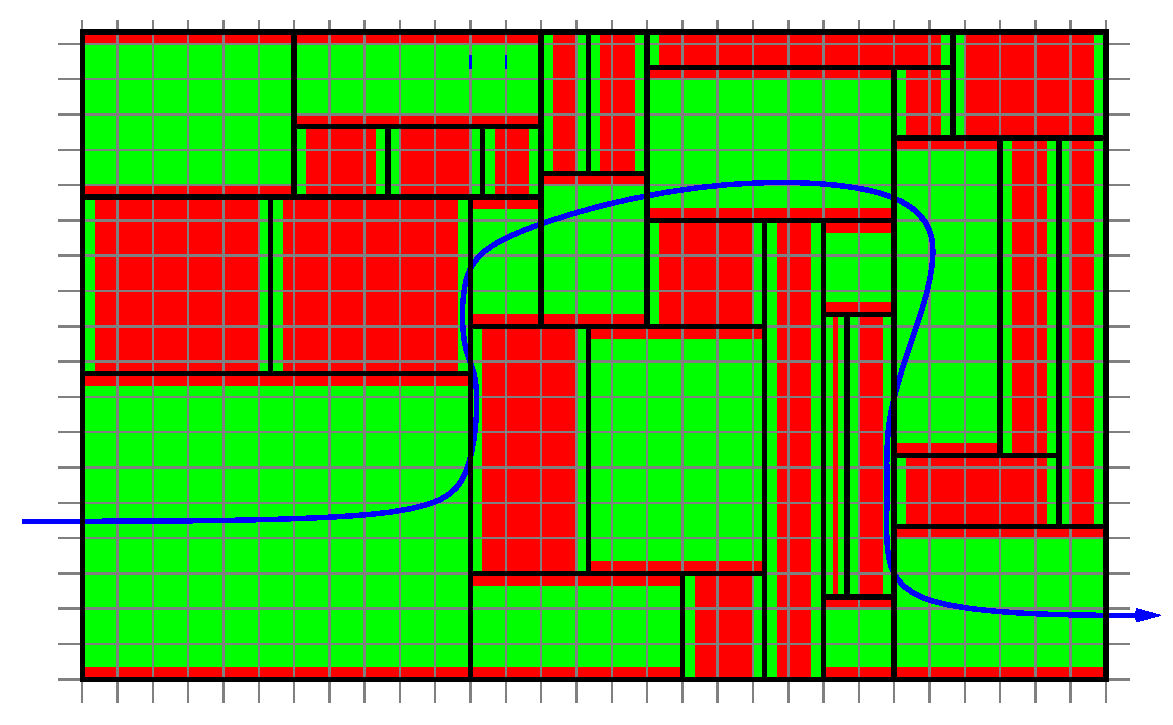
\includegraphics[scale=0.5]{Figs/Insight/green}
\end{figure}

Поместим в нижний левый угол большого прямоугольника начало координат.
Заметим, что у нас есть либо зелёный путь с левой стороны большого прямоугольника до его правой стороны, либо красный путь с нижней стороны до верхней.
Рассмотрим первый вариант.
Каждое место пересечения зелёного пути с вертикальными сторонами малых прямоугольников имеет целую координату; таким образом, основание большого прямоугольника --- целое число.
Подобным же образом и красный путь снизу вверх определяет целую высоту.

\subsubsection*{Весы и гири} %(TIPPING THE SCALES)

Рассмотрим результат для каждого подмножества учеников, включая пустое.
Заметьте, что каждая гиря окажется на левой чашке весов ровно в половине случаев.
В частности, средний вес гирь на левой чашке для всех подмножеств учеников равен их среднему весу на правой чашке.
Поскольку для пустого множества правая чашка тяжелее, 
для какого-то другого множества тяжелее должна быть левая.\heart

\noindent{\small Источник: Вторая Всесоюзная математическая олимпиада, Ленинград, 1968.}

Техника «усреднения», описанная выше, часто используется: будьте внимательны!

\subsubsection*{Часы на столе} %(WATCHERS ON THE TABLE)

Рассматривая только одни часы, 
мы видим, что в течении одного часа среднее расстояние от центра стола $C$ до кончика минутной стрелки $M$ превышает расстояние от $C$ до центра часов $W$.
Действительно, если провести через точку $C$ прямую $L$, перпендикулярную прямой $CW$, 
то среднее расстояние от прямой $L$ до точки $M$, очевидно, равно $LW$, 
что, в свою очередь, равно $CW$.
Но расстояние $CM$, по меньшей мере, равно $LM$, а обычно больше.

Взяв сумму по всем часам, приходим к аналогичному заключению, и отсюда следует, что есть момент в течении одного часа, когда желанное неравенство выполняется.\heart

\begin{figure}[h!]
\centering
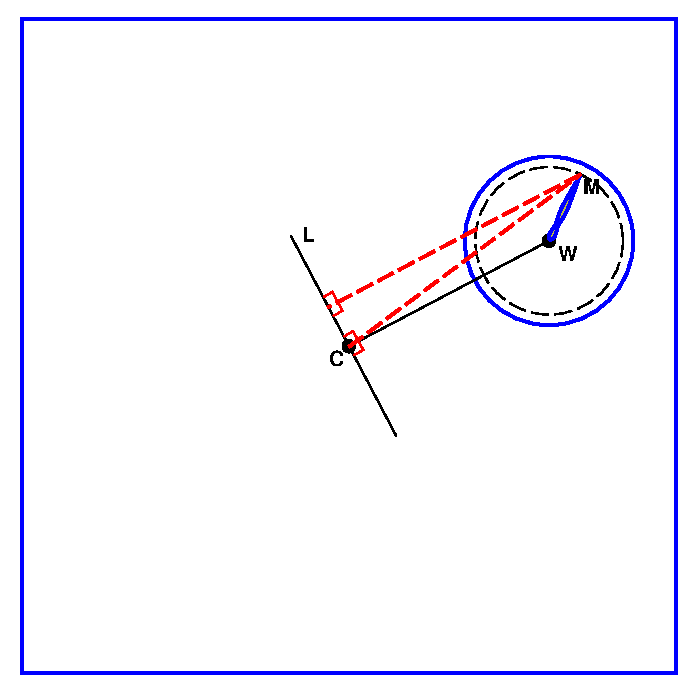
\includegraphics[scale=0.9]{Figs/Insight/watch}
\end{figure}

Требование точности часов обеспечивает движение каждой минутной стрелки с постоянной скоростью.
Это не так уж важно, когда скорости различаются, если только наше терпение не ограничено одним часом.

Одно дополнительное замечание: если установить и расположить часы определённым образом,
то \emph{можно} добиться того, что сумма расстояний от центра стола до кончиков минутных стрелок всегда была строго больше, чем сумма расстояний от центра стола до центров часов.\heart

\noindent{\smallИсточник: данная задача впервые появилась на десятой Всесоюзной математической олимпиаде в Душанбе, 1976.}

\subsubsection*{Путь по шахматной доске} %(PATH ON CHESSBOARD)

Если $n$ --- чётное число, у Боба имеется простая выигрышная стратегия, независимо от того, где Алиса начинает.
Он просто представляет себе, что шахматная доска покрыта прямоугольничками размером $1{\times2}$ клетки (домино) и каждый раз ставит фишку на вторую клетку того домино, куда пошла Алиса («закрывает» домино). %???обычно говорят «доминошки»
(Заметим, что эта стратегия работает для Боба, даже если Алисе разрешено ставить фишку на любую клетку при каждом ходе!).

Если $n$ --- нечётное, и Алиса начинает с угла, она выигрывает, если представит, что домино покрывает всю доску, кроме угловой клетки, с которой она начинает.

Tем не менее, Алиса проигрывает в случае с нечётным $n$, если она должна начинать с клетки, соседней к угловой.
Предположим, угловые клетки на данной доске чёрные, то есть Алиса начинает с белой клетки.
Существует покрытие всей шахматной доски домино, за исключением одной чёрной клетки.
Боб выигрывает, «закрывая» все домино.
Алиса
никогда не сможет поставить фишку на незакрытую клетку, потому что все клетки, на которые она ходит --- белые.\heart

\noindent{\small Источник: Двенадцатая Всесоюзная математическая олимпиада, Ташкент, 1978.}

\subsubsection*{Степень в степени} %(EXPONENT UPON EXPONENT)

Если выражение
$${\sqrt{2}}^{{\sqrt{2}}^{{\sqrt{2}}^{{\cdot}^{\cdot^{\cdot}}}}}$$
имеет какой-то смысл, то это не что иное, как предел последовательности
$${\sqrt{2}}, {\sqrt{2}}^{{\sqrt{2}}}, {\sqrt{2}}^{{\sqrt{2}}^{{\sqrt{2}}}},\dots$$
Этот предел существует, так как последовательность возрастает и ограничена.

Для доказательства первого утверждения, обозначим эту последовательность
$s_1, s_2,\dots$ и докажем по индукции, что $1<s_i\z<s_{i+1}$
для каждого $i\ge 1$.
Это сделать легко, поскольку \[s_{i+2}=
{\sqrt{2}}^{s_{i+1}}
>{\sqrt{2}}^{s_{i}}
=s_{i+1}.\]

Для нахождения верхней грани, заменим самую верхнюю степень в каждом $s_i$ на б\'{о}льшее число $2$, тогда всё выражение превращается в двойку.

Теперь, когда мы знаем, что предел существует, обозначим его $y$.
Он должен удовлетворять уравнению ${\sqrt{2}}^y=y$.
Рассмотрев уравнение $x=y^{1/y}$, 
можно увидеть, применив элементарный матанализ (приношу извинения!), 
что $x$ строго возрастает при возрастании $y$ до максимума при $y=e$
и после чего убывает.
Таким образом, существует не больше двух значений $y$, для данного $x$, 
и при $x=\sqrt{2}$ нам известны оба: $y=2$ и $y=4$.

Поскольку наша последовательность ограничена сверху двойкой, можно исключить $4$ и, таким образом, $y=2$.\heart

Обобщив приведённое выше доказательство, мы видим, что выражение $x^{x^{x^{{\cdot}^{\cdot}}}}$
имеет смысл и равно наименьшему решению уравнения $x=y^{1/y}$ при $x\le e^{1/e}$.
При $x=e^{1/e}$, выражение равно $e$ но как только $x$ превысит $e^{1/e}$, последовательность устремляется к бесконечности.

\subsubsection*{Солдаты в поле}%(SOLDIERS IN THE FIELD)

Данная задача была представлена на шестой Всероссийской математической олимпиаде в Воронеже, 1966.
Её легче всего решать, начав с двух солдат, находящихся друг от друга на кратчайшем расстоянии.
Ясно, что они присматривают друг другом, и если кто-то ещё смотрит на одного из них, тогда у нас имеется солдат, за которым присматривают дважды и, значит, есть солдат, за которым никто не присматривает.
Если же за этими двумя солдатами больше никто не присматривает, то можно их убрать, не влияя на остальных.

Так как число солдат нечётное, то, применяя и далее это рассуждение, мы, в конце концов, придём к одному солдату, который ни за кем не присматривает --- противоречие.\heart

\subsubsection*{Отрезки и расстояния} %(INTERVALS AND DISTANCES)

{\small Источник: Семнадцатая Всесоюзная математическая олимпиада, Кишинёв, 1983.}

Обозначим через $s_1,\dots,s_k$ длины отрезков множества $S$,
пусть их сумма равна $s$.
Рассмотрим интервал $I_{ij}$, содержащий все расстояния, которые можно получить, взяв первую точку на $i$-том и вторую на $j$-том отрезке множества $S$.
Ясно, что длина $I_{ij}$ равна $s_i+s_j$.
Суммируя по всем парам $i\ne j$, 
каждая длина появляется $k-1$ раз,
таким образом, сумма длин интервалов по всем парам различных отрезков, не превосходит $(k-1) s$.
Расстояния между точками, взятыми из $i$-ого отрезка, имеют значения от $0$ до $s_i$.
Значит, общая длина всех интервалов $I_{ij}$ не превосходит $k s$.
Поскольку $k s\ge 1$, получаем $s\ge 1/k$.
\heart

Равенство достигается, если максимум всех $s_i$ равен $s$, 
то есть если все отрезки, кроме одного, имеют нулевую длину.
Этого можно добиться взяв отрезок $[0,\tfrac1k]$ и добавив изолированные точки
$\tfrac2k,\tfrac3k,\dots,1$.

%исправлена фактическая ошибка --- отрезок можно брать только с краю, в середине брать нельзя.

\subsubsection*{Собрать 15} %(SUMMING TO 15)

Быстрый способ решить данную задачу --- это представить, что Алиса и Боб пользуются следующим магическим квадратом:
$$
\begin{matrix}
8&1&6\\
3&5&7\\
4&9&2
\end{matrix}
$$
Так как числа в строчке, столбике и диагонали дают в сумме 15, то можно сказать, что они играют в крестики-нолики! 
Всем известно, что наилучшая игра в крестики-нолики приводит к ничьей,
то есть ответ на наш вопрос --- нет, у Алисы нет выигрышной стратегии.
\heart

Эта забавная игра упоминается во втором томе классической книги Элвина Берлекампа, Джона Конвея и Ричарда Гая.\footnote{Winning Ways for Your Mathematical Plays by Elwyn Berlekamp, John Conway and Richard Guy ; Academic Press, 1982: 2nd Edition, A K Peters 2001}
В книге задача приписывается некоему «Э. Периколозо Спорджерси»\footnote{E. Pericoloso Sporgersi}, что выглядит очень подозрительно --- такую надпись можно увидеть в итальянских поездах, она предупреждает пассажиров об опасности высовываться из окна.

\chapter*{Числа}
\addcontentsline{toc}{chapter}{Числа}

\setlength{\epigraphwidth}{.4\textwidth}
\epigraph{Счастья светлого полны\\ %We learned to be happy,
На балу танцуем мы.\\ % We danced’ round the hall
А причину что скрывать ---\\ %And learning to count was the key to it all.
Научились мы считать.}{Граф фон Знак, «Улица Сезам»}

%The Count, “Sesame Street” 

 

Числа --- это бесконечный источник очарования, а для некоторых --- болезнь на всю жизнь. %кого-то и страсть на всю жизнь.
Бывает, что свойства конкретного числа овладевают умом человека;
про такие числа придумано множество интригующих задач,
часто требующих делать выводы из того, что на первый взгляд кажется нехваткой данных.
%основанных на кажущейся нехватке данных.

Задачи, подобранные здесь, подразумевают % предлагают 
более общий подход. % идею, более универсальный подход.
%Идея задач, подобранных здесь, --- предложить более общий, универсальный подход.
%Дух (spirit) данной коллекции ( Настроение данной коллекции подразумевает) предлагает тем не менее стремление к большей (общности )универсальности.
Наши численно-теоретические задачи о числах в целом, а не только об отдельных, особенных числах.
В ряде случаев для их решения вам понадобится несколько больше, чем знание того, 
что любое натуральное число представляется как произведение простых единственным образом.

\medskip

Вот задача для примера:

\subsection*{Двери шкафчиков}% ДВЕРИ ШКАФЧИКОВ (LOCKER DOORS)
\rindex{Двери шкафчиков}

Шкафчики в раздевалке школьного спортивного зала пронумерованы по порядку от 1 до 100.
Ученик, пришедший первым, открывает все шкафчики.
Второй ученик проходит следом и закрывает все шкафчики с чётными номерами, третий ученик меняет положение дверей у шкафчиков с номерами, кратными 3.

Так продолжается до тех пор, пока не пройдёт сотый ученик.
Какие шкафчики будут после этого открыты?
 
\paragraph{Решение:}

Состояние $n$-го шкафчика (открыт-закрыт) изменяется, когда проходит $k$-тый ученик, если $k$ --- делитель числа $n$.
Обычно, делители можно разбить на пары $\{j,k\}$, где $j\cdot k=n$.
Таким образом, совокупный эффект от учеников $j$ и $k$ на данную дверь отсутствует. %будет равен 0.
Но, если $n$ --- совершенный квадрат, то нет другого делителя, отменяющего действия $\sqrt{n}$-го ученика.
Следовательно, в конце будут открыты только шкафчики, номера которых являются совершенными квадратами: 1, 4, 9, 16, 25, 36, 49, 64, 81 и 100.\heart
 
В начале раздела мы сделаем пару наблюдений, касающихся представления целых чисел в десятичной системе счисления, и закончим неожиданно хитрой головоломкой для ужина с друзьями. % (surprisingly subtle dinner table conundrum).

\subsection*{Нули, единицы и двойки}% НУЛИ, ЕДИНИЦЫ И ДВОЙКИ. (ZEROES, ONES AND TWOS)
\rindex{Нули, единицы и двойки}

Пусть $n$ --- натуральное число.
Докажите, что (а) существует число кратное $n$ (не равное нулю), чьё представление в десятичной системе содержит только нули и единицы, и
(б) существует число кратное $2^n$, состоящее только из единиц и двоек.

\subsection*{Суммы и разности} %СУММЫ И РАЗНОСТИ (SUMS AND DIFFERENCES)
\rindex{Суммы и разности}

Даны 25 положительных чисел.
Докажите, что можно выбрать из них два числа, так, что ни одно из оставшихся чисел не равно ни их сумме, ни их разности.

\subsection*{Генерирование рациональных чисел}%??? Получение ГЕНЕРИРОВАНИЕ РАЦИОНАЛЬНЫХ ЧИСЕЛ (GENERATING THE RATIONALS)
\rindex{Генерирование рациональных чисел}

Множество $S$ содержит 0 и 1, а также средние значения всех конечных непустых подмножеств множества $S$.
Докажите, что $S$ содержит все рациональные числа единичного отрезка.

\subsection*{Суммирование дробей}%СУММИРОВАНИЕ ДРОБЕЙ ( SUMMING FRACTIONS )
\rindex{Суммирование дробей}

Дано натуральное число $n>1$, 
сложите все дроби $1/pq$, где $p$ и $q$ взаимно простые числа при $p+q>n$ и $0<p<q\le n$.
Докажите, что результат суммирования всегда равен $1/2$.

\subsection*{Вычитания по кругу}
%ВЫЧИТАЯ ПО КРУГУ (SUBTRACTING AROUND THE CORNER)
\rindex{Вычитания по кругу}

Напишите последовательность из $n$ положительных чисел.
Замените каждое из чисел на модуль разности %(absolute difference) 
этого и следующего по кругу за ним числа.
Повторяйте до тех пор, пока все числа станут равны нулю.
Докажите, что для $n=5$ этот процесс может продолжаться бесконечно, 
а при $n=4$ он всегда закачивается.

\subsection*{Прибыли и убытки}%ПРИБЫЛИ И УБЫТКИ (PROFIT AND LOSS)
\rindex{Прибыли и убытки}

На совещании акционеров правление представило помесячный отчёт о прибылях (либо об убытках) сo времени проведения последнего собрания.
«Заметьте, --- сказал генеральный директор,--- за каждые идущие подряд восемь месяцев мы получали прибыль»
«Может быть и так, --- посетовал один из акционеров, --- но я также вижу, что за каждый период из последовательно идущих пяти месяцев мы несли убытки!»

Какое максимальное число месяцев могло пройти сo времени проведения последнего собрания?

\subsection*{Первое нечётное число в словаре}%ПЕРВОЕ НЕЧЁТНОЕ ЧИСЛО В СЛОВАРЕ (FIRST ODD NUMBER IN THE DICTIONARY)
\rindex{Первое нечётное число в словаре}

Представьте, числа от 1 до $10^{10}$ записаны формальным русским языком (например, «двести одиннадцать» или «одна тысяча сорок два») и затем расставлены в алфавитном порядке (как в словаре, буква за буквой, пробелы и дефисы игнорируются).
Какое нечётное число встретится первым?

%ё
\section*{Решения и комментарии}

\subsubsection*{Нули, единицы и двойки}%НУЛИ, ЕДИНИЦЫ И ДВОЙКИ (ZEROES, ONES AND TWOS) 

Для части a) мы применим знаменитый и полезный принцип ящиков Дирихле:
Если число голубей больше числа ящиков, то хотя бы в одном из ящиков находится более одного голубя.

Мы знаем, что существует только $n$ различных остатков от деления на $n$, а множество $\{1, 11, 111, 1111,\dots\}$, чей наибольший элемент
состоит из $n+1$ цифр, содержит $n+1$ членов.
Следовательно, в нём содержатся два числа, имеющих одинаковый остаток при делении на $n$. 
Отнимите одно от другого!
\heart

Дэвид Гейл %(David Gale) 
указал мне на то, %обратил моё внимание на то, 
что если $n$ не делится на 2 и 5, то можно найти число кратное $n$, представляемое (в десятичной системе) одними единицами. 
Действительно, приведённое выше доказательство выдаёт нам число вида $111\dots111000\dots000$; 
если у нас на конце $k$ нулей, то деление на $10^k=2^k\cdot 5^k$ оставляет нам число из одних единиц и всё ещё кратное $n$. 

В части (б) легче всего, применить индукцию по $k$
и доказать, что существует число из $k$ цифр, кратное $2^k$ и состоящее только из единиц и двоек.
Добавление 1 или 2 в начало такого числа увеличит его на $2^k5^k$ или $2^{k+1}5^k$, в обоих случаях сохраняется делимость на $2^k$. 
Так как два полученных числа отличаются на $2^k5^k$, одно из них должно делится на $2^{k+1}$.
\heart

Первая задача попала ко мне от Муту Мутукришнана %(Muthu Muthukrishnan) 
из отдела исследований AT\&T и Ратгерского университета. 
Вторая была представлена на пятой Всесоюзной математической олимпиаде в Риге в 1971 году. 
Приведённое здесь решение принадлежит Саше Баргу %(Sasha Barg) 
из Мэрилендского университета.

\medskip

В похожей задаче на первой Всесоюзной математической олимпиаде в Тбилиси в 1967 году требовалось доказать, что существует число, которое делится на $5^{1000}$ и в своей десятичной записи не содержит ни одного нуля. 
Один способ --- это доказательство от противного, 
пусть $k$ --- наибольшая возможная степень пятёрки.
Пусть $n$ есть кратное наибольшей степенью пятёрки (скажем $5^j$ при $j\le k$)
среди всех $k$-значных чисел.
Тогда $n\equiv d\cdot 5^j\pmod{5^{j+1}}$ для некоторого $0<d<5$.
Отняв от $n$ число $d\cdot 10^{j+1}$ или прибавив к нему $(5-d)\cdot 10^{j+1}$
мы получим число без нулей и улучим его делимость --- противоречие.
\heart

\subsubsection*{Суммы и разности}%СУММЫ И РАЗНОСТИ (SUMS AND DIFFERENCES) 

Данная задача была также представлена на пятой Всесоюзной математической олимпиаде в Риге, 1971.

\medskip

Упорядочим числа $x_1<x_2<\dots<x_n$ (мы полагаем $n=25$ нам потребуется только, что $n$ нечётно).
Если $x_n$ не является одним из искомых чисел, значит для каждого меньшего числа $x_i$ существует другое число $x_j$, такое что $x_i+x_j=x_n$.
Таким образом первые 24 числа разбиваются на пары и значит $x_i+x_{n-i}=x_n$ для любого $i$.

Сумма $x_{n-1}$ с любым из чисел $x_2,\dots,x_{n-2}$ больше, чем $x_n=x_1+x_{n-1}$.
Значит, если $x_{n-1}$ не является одним из искомых чисел, то для каждого числа $x_i$ из $x_2,\dots,x_{n-2}$ есть пара $x_j$, что 
$x_{i}+x_{j}=x_{n-1}$.
Отсюда $x_{i}+x_{n-1-i}=x_{n-1}$ для каждого $i$.
Однако в этом случае $x_{(n-1)/2}$ парно самому себе, 
и значит пара $x_{n-1}$, $x_{(n-1)/2}$ является решением нашей задачи --- противоречие.
\heart 

\subsubsection*{Генерирование рациональных чисел}%ГЕНЕРИРОВАНИЕ РАЦИОНАЛЬНЫХ ЧИСЕЛ (GENERATING THE RATIONALS) 

В первую очередь заметим, что множество $S$ содержит все двоично-рациональные числа, 
то есть дроби вида $p/2^n$. 
Все такие числа со знаменателем $2^n$ и нечётным числителем мы можем получить, взяв среднее значение двух соседних чисел со знаменателями меньшей степени. 

Любая дробь $p/q$, очевидно, является средним $p$ единиц и $q-p$ нулей. 
Выберем $n$ достаточно большим и заменим все нули на $1/2^n$, $-1/2^n$, $2/2^n$, $-2/2^n$, $3/2^n$ и так далее, включая один $0$, если $p$ нечётное. 
Подобным же образом заменим единицы на $1-1/2^n$, $1+1/2^n$, $1-2/2^n$, $1+2/2^n$ и так далее. 
Конечно, некоторые из этих чисел находятся вне единичного отрезка, но можно повторить то же рассуждение для интервала между двоично-рациональными числами содержащего $p/q$ и лежащего строго в единичном отрезке.%(rescale the procedure to fit some dyadic interval)
\heart

Источник: Тринадцатая Всесоюзная математическая олимпиада, Тбилиси, 1979.   

\subsubsection*{Суммирование дробей}%СУММИРОВАНИЕ ДРОБЕЙ ( SUMMING FRACTIONS ) 

Проведём доказательство по индукции, заметив, что высказывание верно для $n=2$.
При переходе от $n$ к $n+1$ мы добавляем $1/pn$ для каждого $p$ с $(p,n)=1$ и теряем $1/pq$ для пар $p$ и $q$ таких, что $(p,q)=1$ и $p+q=n$.
Таким образом, каждая пара, удовлетворяющая условию задачи, означает потерю $1/pq$, и добавление $1/pn+1/qn=1/pq$, а значит результат не меняется.\heart
%(neatly cancelling).

Источник: Третья Всесоюзная математическая олимпиада, Киев, 1969. 

\subsubsection*{Вычитания по кругу}%ВЫЧИТАЯ ПО КРУГУ (SUBTRACTING AROUND THE CORNER) 

Один внештатный преподаватель математики старших классов (средняя школа в Фер Лон, Нью-Джерси, 1962)
%(Fair Lawn Senior High School) 
рассказывал мне,
что некоторые военнопленные Второй Мировой войны развлекались тем, что брали различные наборы из четырёх чисел и смотрели как долго они могут прокручивать эту операцию. 

\medskip

Обе задачи решаются рассмотрением процесса по модулю 2.
Для $n=4$ с точностью до циклических перестановок и симметрий, 1 0 0 0 и
1 1 1 0 становятся 1 1 0 0, затем 1 0 1 0, затем 1 1 1 1 и затем 0 0 0 0.
Поскольку здесь охватываются все случаи, мы видим, что при работе с обычными целыми числами нам понадобится не более 4 шагов, чтобы все они стали чётными, и на этом этапе, до того, как продолжить далее, мы можем поделить их на двойку в наибольшей общей степени. 
Так как самое большое в последовательности число $M$ не может увеличиваться и уменьшается в два раза или более хотя бы один раз за каждые четыре шага, 
мы приходим к 0 0 0 0 максимум за $4(1+\lceil\log_2 M\rceil)$ шагов.

С другой стороны, при $n=5$ последовательность 1 1 0 0 0 (рассматриваемая как последовательност бинарных или обычных чисел)
проходит по циклу 
1 0 1 0 0, 
1 1 1 1 0, 
1 1 0 0 0.\heart 

Несложный анализ, использующий многочлены над целыми по модулю два, показывает, что всё зависит от того является ли $n$ степенью двойки. 

\subsubsection*{Прибыли и убытки}%ПРИБЫЛИ И УБЫТКИ (PROFIT AND LOSS) 

Данная задача представляет собой адаптированный вариант задачи, предложенной одним вьетнамским автором на Международной Математической Олимпиаде 1977 года. 
Мне её рассказал Титу Андрееску, %(Titu Andreescu), 
за что я ему очень благодарен. 
Решение, однако, моё собственное. 

Нам нужна, конечно, последовательность чисел максимальной длины, такая, что сумма чисел каждой подстроки длины 8 --- больше нуля, а сумма чисел каждой подстроки длины 5 --- меньше нуля. Строка, без сомнения, должна быть конечной, более того, длиной меньше 40, иначе вы могли бы выразить сумму первых 40-ка членов и как (положительную) сумму 5 подстрок длины 8, и как сумму (отрицательную) 8 подстрок длины 5.  

Давайте решим эту задачу в более общем виде. Пусть $f(x,y)$ --- длина максимальной строки, такой, что сумма каждой $x$-подстроки положительна, а сумма каждой $y$-подстроки --- отрицательна. 
Мы можем предположить, что $x>y$. 
Если $x$ кратно $y$, тогда $f(x,y)=x-1$ --- мы должны согласиться, что это утверждение верно по отношению к $x$-подстрокам за отсутствием таковых. 

Что, если $y=2$ и $x$ --- нечётное?
Тогда можно построить строку длины $x$ с чередующимся элементами, скажем, $x-1$ и $-x$. 
Однако такой строки длины $x+1$ не существует.
Действительно, в каждой $x$-подстроке нечётный элемент должен быть положительным 
(так как можно покрыть всю $x$-подстроку 2-подстроками за исключением произвольного нечётного элемента). 
Для двух $x$-подстрок, это означает, что все элементы положительны ---
противоречие.  

Рассуждение выше подсказывает, что $f(x,y)\le x+y-2$, если $x$ и $y$ взаимно просты, 
то есть не имеют общего делителя отличного от~1. 
Докажем это по индукции. 
Рассуждая от противного, предположим что $f(x,y)\ge x+y-1$;
то есть имеется строка длины $x+y-1$, удовлетворяющая указанным условиям. 
Положим $x=ay+b$, где $0<b<y$. 
Заметим, что каждая $b$-подстрока %(any consecutive b of them) 
может быть представлена как $x$-подстрока полной строки, 
без $a$ штук $y$-подстрок; 
следовательно, сумма в любой $b$-подстроке положительна. 
Отсюда
$f(b,y)\ge x+y-1$,
что противоречит предположению индукции поскольку $y$ и $b$ взаимно просты и $b<y<x$.

Чтобы показать, что $f(x,y)=x+y-2$, когда $x$ и $y$ взаимно просты, мы построим $(x+y-2)$-строку, обладающую требуемыми свойствами.
Более того, числа нашей строки будут принимать ровно два различных значения $u$ и $v$,
а также строка будет периодической с двумя периодами $x$ и $y$. 

Представим себе, что мы расставили $u$ и $v$ их произвольным образом в первой $y$-подстроке.
Продолжим расстановку, заставляя строку быть периодической с периодом $y$.
Чтобы добиться того же с периодом $x$,
нам нужно обеспечить, чтобы последние $y-2$ элементов соответствовали первым.
Это условие можно записать как $y-2$ равенств на $y$ значений выбранных нами изначально. 
Поскольку этих равенств недостаточно, чтобы заставить все решения быть одинаковыми, мы можем гарантировать, что существует по меньшей мере одно $u$ и одно $v$.

Проделаем это для $x=8$ и $y=5$.
Пусть $c_1\dots c_5$ будут первые пять элементов строки, 
таким образом вся строка будет выглядеть как
$c_1c_2c_3c_4c_5c_1c_2c_3c_4c_5c_1$. 
Для того, чтобы строка была периодична с периодом 8, 
нужно потребовать $c_4=c_1$, $c_5=c_2$ и $c_1=c_3$. 
Значит можно считать $c_1=c_3=c_4=u$ и $c_2=c_5=v$; 
тем самым получается последовательность $uvuuvuvuuvu$. 

Возвращаясь к задаче в общем виде, 
заметим, что строка с периодом $x$ автоматически обладает следующим свойством: сумма каждой $x$-подстроки одна и та же, потому как, каждый раз, когда вы сдвигаете $x$-подстроку на один шаг, элемент, приобретённый на одном конце, такой же, как и элемент, потерянный на другом.
Конечно, это высказывание справедливо и для $y$-подстрок, если строка периодична с периодом $y$.

Пусть $S_x$ --- сумма $x$-подстроки, a $S_y$ --- сумма $y$-подстроки. 
Заметим, что $S_x/x\ne S_y/y$.
Это объясняется тем, что, если у нас $u$ встречается в каждой
 $x$-подстроке, скажем, $p$ раз, а $v$, в каждой $y$-подстроке --- $q$ раз, 
 то равенство $S_x/x=S_y/y$
 означало бы 
\[y(pu+(x-p)v)=x(qu+(y-q)v)\]
что сводится к $yp=xq$ так как $u\ne v$. 
Поскольку $x$ и $y$ взаимно простые, этого не может быть при $0<p<x$ и $0<q<y$. 

Отсюда следует, что можно подобрать $u$ и $v$ так, чтобы сумма $S_x$ была положительна, а $S_y$ отрицательна. 
Например, в случае, рассматриваемом выше, каждая 8-подстрока содержит пять $u$ и три $v$, 
а в свою очередь, каждая 5-подстрока имеет три $u$ и две $v$.
Если взять $u=5$ и $v=-8$, то получим $S_x=1$ и $S_y=-1$. 
Итак, решением исходной задачи будет последовательность $5,-8,5,5,-8,5,-8,5,5,-8,5$.
\heart

Усердный читатель легко обобщит вышеприведённое доказательство на случай, 
когда наибольший общий делитель $x$ и $y$ отличнен от~1. 
Результат будет $f(x,y)=x+y-1-\text{НОД}(x,y)$.    

\subsubsection*{Первое нечётное число в словаре}%ПЕРВОЕ НЕЧЁТНОЕ ЧИСЛО В СЛОВАРЕ (FIRST ODD NUMBER IN THE DICTIONARY) 

Решение данной задачи --- всего лишь вопрос внимательного и методичного рассмотрения последовательности слов, составляющих числительные.
Самое первое число будет, конечно, «восемнадцать», и первое идущее за ним слово (можем считать его как бы суффиксом) --- «миллионов».
Итак, искомое число должно начинаться с «восемнадцать миллионов», следуя подобным образом далее, мы получаем окончательный ответ какой 18 018 089 --- «восемнадцать миллионов восемнадцать тысяч восемьдесят девять».%
\footnote{Ответ в оригинальной задаче на английском языке выглядит похоже: 8,018,018,885 --- «eight billion eighteen million eighteen thousand eight hundred eighty-five».}
\heart

Идея этой забавной задачи пришла ко мне после того, как Херб Уилф из Пенсильванского университета %(Herb Wilf, University of Pennsylvania) 
попросил меня назвать первое простое число в словаре. 
Автором этого вопроса считается компьютерный гуру из Стэндфордского университета Дональд Кнут. %(Donald Knuth, Stanford University).
Рассуждая так же как и выше, с проверкой простоты числа на компьютере
получаем, что ответ равен 18 018 881.%
\footnote{На английском, это будет 8,018,018,881 --- «eight billion eighteen million eighteen thousand eight hundred eighty-one».}


\chapter*{Комбинаторика}
\addcontentsline{toc}{chapter}{Комбинаторика}

\setlength{\epigraphwidth}{.6\textwidth}
\epigraph{Ложь имеет бесконечное число комбинаций,
тогда как правда бывает только одна.}{Жан-Жак Руссо}

 
 
Если задача начинается со слов «Сколько существует способов...», то это автоматически задача по комбинаторике, но обратное неверно.
Комбинаторный подход будет полезен при решении как нижеследующих (довольно разнообразных) задач, так и многих других в этой книге.

Наша вводная задача совершенно классическая и использует фундаментальную
комбинаторную технику --- перемножение чисел независимых вариантов.

\subsection*{Расстановка цифр}% (Sequencing the Digits)
\rindex{Расстановка цифр}

Сколькими способами можно записать в ряд цифры от 0 до 9, так, что каждая цифра, кроме самой левой, отличается от одной из цифр стоящих слева от неё, на единицу.

\paragraph{Решение:} На первый взгляд кажется, что данная задача не решается перемноженим чисел независимых вариантов, так как число вариантов зависит от предыдущего выбора.
Например, у нас есть десять вариантов для самой левой цифры,
но начав ряд, скажем, с «3» у нас только два варианта для следующей цифры; если же мы начинаем с «0» или «9», то у нас только один выбор.
Если вы знаете как суммировать биномиальные коэффициенты, то вы можете построить на этом решение задачи, но есть лучший способ.

Заметим, что ряд заканчивается нулём или девяткой; и если мы движемся \emph{справа налево}, то каждый раз мы стоим перед выбором --- написать наибольшую неиспользованную цифру или наименьшую, пока не дойдём до левого края, где эти два выбора совпадают.
Таким образом, получаем два выбора в каждой из девяти возможностей.
Отсюда ответ $2^9=512$ способов.\heart

(Источник: Олимпиада Патнема 1960-х годов.)% (A Putman Exam from the 1960s )

\bigskip

За вами решение оставшихся задач.
Подсказка: смотрите внимательно, где можно применить принцип Дирихле!

\subsection*{Подмножества подмножеств}% (Subsets of subsets)
\rindex{Подмножества подмножеств}

Докажите, что любое множество из десяти различных чисел от 1 до 100 содержит два непересекающихся непустых подмножества, сумма чисел которых одинакова.

\subsection*{Вредный метрдотель}% (The Malicious Maitr D’)
\rindex{Вредный метрдотель}

На банкете математической конференции 48-ми мужчинам математикам, ни один из которых не имеет ни малейшего представления об этикете, назначены места за большим круглым столом.
На столе, между каждой парой приборов, стоит кофейная чашка с салфеткой.
Как только человек занимает своё место (по указанию метрдотеля), он берёт салфетку, слева или справа от себя; если на столе две салфетки, он выбирает одну случайным образом (но метрдотель не может видеть, какую).

В каком порядке следует заполнять места, чтобы максимальному числу математиков не досталось салфетки?

\subsection*{Рукопожатия на приёме}% (Handshakes at a Party)
\rindex{Рукопожатия на приёме}

Майк и Жанна, а также ещё четыре пары, побывали на праздничном обеде, где каждый из присутствующих обменялся рукопожатием с каждым, ему дотоле незнакомым гостем.
Позже Майк опросил всех и обнаружил, что каждый из девяти других гостей пожал руки с \emph{разным} числом людей.

Со сколькими гостями обменялась рукопожатиями Жанна?

\subsection*{Трёхсторонние выборы}% (Three-Way Election)
\rindex{Трёхсторонние выборы}

Ашворд, Бакстер и Кэмпбелл баллотируются на пост председателя союза %(secretary of union) 
и набирают по одинаковому числу голосов.
Для разрешения этой ситуации они требуют голосования с учётом второго выбора избирателей (так называемого преференциального метода голосования), но снова приходят к ничьей.
Тогда Ашворд выступает с предложением, что, так как число избирателей нечётное, можно провести двухсторонние выборы --- избиратели выбирают между Бакстером и Кэмпбеллом, а затем между победителем и Ашвордом.

Но Бакстер недоволен данным предложением.
Он считает этот способ несправедливым, потому что, по его мнению, у Ашворда больше шансов выиграть, чем у остальных.
Прав ли Бакстер?

\subsection*{Зарплата короля}% (King’s Salary)
\rindex{Зарплата короля}

После революции каждый из 66 жителей некой страны, включая короля, получает зарплату в 1 доллар.
Король не может больше голосовать, но всё ещё сохраняет за собой право вносить изменения в законопроект, в частности, в то, как распределяется зарплата.
Зарплата каждого жителя должна быть целым числом долларов и сумма всех зарплат равняется 66.
Каждое предложение по изменению ставится на голосование и принимается, если получает больше голосов «За», чем «Против».
Будем считать, что те, кто получают прибавку к зарплате, голосуют «За», а те, у кого зарплата уменьшается --- «Против», остальные же голосованием себя не утруждают.

Король --- человек умный и корыстный.
Какой максимальной для себя зарплаты он может добиться, и сколько шагов ему на это понадобится?

\subsection*{Плохо сделанные часы}% (A Poorly Designed Clock)
\rindex{Плохо сделанные часы}

Есть часы, у которых минутная стрелка никак не отличается от часовой.
Сколько раз в сутки возникнет ситуация, когда по этим часам нельзя определить время в данный момент?

\subsection*{Таинственный карточный фокус}% (A Mystifying Card Trick )
\rindex{Таинственный карточный фокус}

Давид и Дороти придумали хитрый карточный фокус.
Давид отворачивается, кто-нибудь выбирает пять карт из колоды карт для бриджа и даёт их Дороти; она просматривает карты, вытаскивает одну и передаёт оставшиеся карты Давиду.
Давид правильно называет вытащенную Дороти карту.

Как они это делают?
На какой наибольшей колоде возможно демонстрировать их фокус?

\subsection*{Странствующие торговцы}% (Travelling Salesmen )
\rindex{Странствующие торговцы}

Между любыми двумя большими городами в России цена авиабилетов фиксирована.
Алексей Фругаль, коммивояжёр, начинает свою поездку по городам из Москвы и всегда выбирает самый дешёвый перелёт до города, который он ещё не посещал.
(Ему не нужно каждый раз возвращаться в Москву).
Коммивояжёру Борису Лавишу также нужно посетить каждый город, но он начинает свою поездку в Калининграде и каждый раз выбирает самый дорогостоящий перелёт до города, в котором он ещё не побывал.

Докажите, что поездки Лавиша стоят как минимум столько же, сколько поездки Фругаля. %???Фругаль = Скряга, Лавиш=Кутила

\subsection*{Проигрыш в кости}% (Losing at Dice)
\rindex{Проигрыш в кости}

При броске шести кубиков, число различных выпавших чисел варируется от 1 до 6.
Предположим, что каждую минуту крупье бросает шесть кубиков,
и вы ставите 1 доллар, один к одному, на то, что выпадет ровно 4 различных числа
(то есть вы получаете 1 доллар, если выигрываете или теряете 1 доллар, если проигрываете).

Если вы начинаете игру с 10 долларами, приблизительно, сколько вы в среднем продержитесь до полного проигрыша?

\section*{Решения и комментарии}

\subsubsection*{Подмножества подмножеств}% (Subsets of subsets)

Хитрость в данной задаче, основанной на одном из заданий Международной математической олимпиады 1972 года, заключается в том, что вначале условие непересечения подмножеств игнорируется, и рассматриваются все подмножества.

\medskip

Множество $S$ из $10$ элементов содержит, разумеется, $2^{10} - 1 \z= 1023$ непустых подмножества.
Могут ли все суммы чисел этих подмножеств быть различными?
Максимальная сумма подмножества множества из десяти чисел от 1 до 100 будет 
$100+99+\dots+91\z<1000$, а минимальная, очевидно, равна 1; таким образом, согласно принципу Дирихле, должны существовать два различных подмножества $A\subset S$ и $B\subset S$ 
с одинаковой суммой.
Конечно, $A$ и $B$ могут пересекаться, но можно просто выбросить общие элементы;
$A\backslash B$ (множество элементов $A$, не содержащихся в $B$) и $B\backslash A$ \emph{не} пересекаются и по-прежнему имеют одинаковую сумму.\heart

\subsubsection*{Вредный метрдотель}% (The Malicious Maitr D’)

Появление данной задачи связано со следующим событием:
30 марта 2001 года принстонский математик Джон Хортон Конвей %(John H. Conway) 
прибыл года в лаборатории Белла, %(Bell Labs) 
чтобы сделать доклад на «Общенаучном семинаре». %(“General Research Colloquium”).
На обеде ваш автор оказался сидящим за столом между Конвейем и специалистом по компьютерным технологиям Робом Пайком %(Rob Pike) 
(сейчас работает в Гугле), и салфетки, и кофейные чашки были расставлены точно так же, как описано в задаче.
Конвей задался вопросом, а сколько человек из
сидящих за столом остались бы без салфеток, если бы их рассаживали в \emph{случайном} порядке (см. Главу 11), а Пайк сказал: «А вот более лёгкий вариант: а какой порядок \emph{самый плохой}?»

\bigskip

Допустим, что метрдотель, когда сажает человека на место, видит, которую салфетку взяли (такого игрока называют «адаптивным противником»). %(“adaptive adversary”) 
Тогда лучшая для него стратегия состоит в следующем:
если первый гость возьмёт салфетку, скажем, справа от себя, то следующий будет посажен на второе место справа, так что тот, кто окажется между ними, может попасть в западню.
Если второй человек берёт салфетку справа, то метрдотель пытается делать то же самое и дальше, пропуская одно место справа.
Если же второй человек возьмёт салфетку слева (оставляя, таким образом, место между ним и первым посаженным без салфеток), то третий сажается сразу справа от второго.
Далее гостям указываются места соответственно этому правилу, пока круг не замкнётся, и тогда последние обедающие (обречённые остаться без салфеток) садятся за стол.
В результате в среднем, $1/6$ часть гостей остаётся без салфеток.

Когда же, как в поставленной задаче, метрдотель не «адаптивный противник», то, как показалось Пайку и мне, правильной стратегией было бы заполнить сначала все чётные, а затем нечётные места.
Для каждого нечётного гостя вероятность остаться без салфетки будет равна $1/4$, %(for an overall yield) 
а конечным результатом будет $1/8$ (то есть 6 из 48 обедающих, в среднем).

Хотя, если подумать ещё немного, то наилучшая стратегия для метрдотеля --- заполнить сначала места с номерами $0\pmod4$, затем нечётные места, и, наконец места $2\pmod4$.
Это расстроит $9/64$ гостей, в среднем.
Чтобы понять это, назовём гостя «одиноким», если, когда он посажен на место, у него ещё нет соседа ни справа, ни слева.
Можно предположить, что все «одинокие» гости рассаживаются первыми, и заметим, что между каждой сидящей подряд парой «одиноких» будет максимум один бессалфеточный гость.

Допустим, два последовательно сидящих «одиноких» гостя находятся на расстоянии $d$ друг от друга (то есть между ними $d-1$ стульев).
Эти места будут заполняться с обеих сторон.
Предположим, последний садящийся между ними человек находится на расстоянии $a$ от правого и на расстоянии $b$ от левого «одинокого» гостя, где $a+b=d$.
Правая салфетка будет уже взята, если только «одинокий» обедающий не сидит сразу справа от него, и все последующие гости между парой «одиноких» не выбрали левые салфетки.
Это случается с вероятностью $1/2^a$.
Таким образом, оказавшийся в ловушке 
гость проигрывает (остаётся без салфетки) с вероятностью
\[(1-2^{-a})(1-2^{-b})=1 + 2^{-d}-2^{-a}-2^{-b},\]
которая минимальна, когда $a$ и $b$ равны или отличаются на 1.

Если «одинокие» гости рассажены на расстоянии $d$ друг от друга, то мы получаем одного потенциального проигравшего на $d$ человек.
Таким образом, если число гостей $n$ кратно $d$, то среднее число проигравших равно $(n/d)(1-2^{-\lfloor d/2\rfloor})(1-2^{-\lceil d/2\rceil})$.
Легко проверить, что эта величина достигает максимума не при $d=2$, где она будет равна $n/8$, а при $d=4$, где получаем $9n/64$.
\heart

\subsubsection*{Рукопожатия на приёме}% (Handshakes at a Party)

Данная задача на старую избитую тему --- на первый взгляд, нам кажется что предоставлено недостаточно информации.
С чего, казалось бы, можно сказать что-то о \emph{Жанне}?
Ответом, в конечном итоге, окажется то, что Жанна в паре с тем, кто не принимал участия в опросе.

Так как для каждого гостя максимальное число рукопожатий будет равно 8, 
девять ответов, полученных Майком, --- это как раз числа от 0 до 8.
Два человека (скажем, $A$ и $B$), ответившие 0 и 8, должны быть парой, ведь в противном случае наличие и отсутствие рукопожатия между ними противоречило бы одному из их ответов.
Теперь проверим $C$ и $D$, которым соответствуют 1 и 7;
поскольку $C$ должен был пожать руки с $B$, а $D$ должен был пропустить $A$, то, применяя рассуждение выше, получаем, что $C$ и $D$ так же являются парой.

Аналогично, гости, ответившие 2 и 6, 3 и 5 также должны быть парами.
Значит Майк и Жанна пожали руки гостям, с б\'{о}льшим результатом опроса;
то есть, каждый из них пожал руку четырём.
\heart

Если вы не нашли доказательства, но догадались, что ответ~4, то ваша интуиция была права.
Если предположить что задача имеет единственный ответ (скажем $x$), то в силу симметрии $x=4$.
Предположим, что (по какой-то причине) каждая пара пожала руки друг-другу, и Майк спросил каждого скольким гостям тот \emph{не} пожал руку.
Тогда Женни должна была пожать $x+1$ рук.
Но смена местами роль рукопожатий и нерукопожатий влечёт, что $x+(x+1)=9$.

Тот факт, что головоломка имеет единственное решение часто оказывается полезным.
В одной из своих «Математических игр» для \emph{Scientific American}, Мартин Гарднер спросил:
Предположим дырка длиной в 6 дюймов просверлена через центр шара, чему равен оставшийся объём?

Может показаться, что для решения задачи необходимо знать диаметр дырки, или диаметр исходного шара, но на самом деле этого не нужно.
Чем больше шар тем шире должна быть дырка, для того чтобы иметь длину 6 дюймов;
при этом вычисления показывают, что объём оставшегося кольца не меняется.

Однако нет необходимости делать эти вычисления если поверить, что решение единственно.
Ответ должен быть то же для шара с 6 дюймами в диаметре и без дырки, а именно $\tfrac43\pi3^3=36\pi$ кубических дюймов.

\subsubsection*{Трёхсторонние выборы}% (Three-Way Election)

Бакстер прав, более того, он недооценивает ситуацию.
Представим себе, что никто из голосующих не изменяет своего выбора, тогда несомненно выигрывает Ашворд!
Предположим, что избиратели, голосовавшие за Ашворда, предпочитают Бакстера Кэмпбеллу (то есть Бакстер выиграет у Кэмпбелла в предложенных двухсторонних выборах).
Тогда избиратели, голосовавшие за Бакстера, должны предпочитать
Кэмпбелла Ашворду, иначе Кэмпбелл не набрал бы $1/3$ голосов второго выбора.
Аналогично, избиратели, голосовавшие за Кэмпбелла, предпочитают Ашворда
Бакстеру.
Таким образом, в нашем случае, Ашворд побеждает Бакстера во втором
голосовании.

Если же избиратели, голосовавшие за Ашворда, предпочитают Кэмпбелла Бакстеру, то симметричное рассуждение приводит нас к тому же результату --- во втором голосовании побеждает Ашворд.
\heart

Эта задача, придумана Эхудом Фридгутом %(Ehud Friedgut)
для работы в классе;
она указывает на то, что разрешение ничьи не так уж просто, как кажется на первый взгляд!

\subsubsection*{Зарплата короля}% (King’s Salary)

Данная задача придумана Йоханом Вестлундом %(Johan Waestlund) 
из Линчёпингского университета, а идея её была навеяна историческими событиями в Швеции.
Тут нужно сделать два важных замечания: (1) король должен временно отдать свою зарплату, чтобы начать эту игру, и (2) на каждом шаге следует уменьшать число жителей, получающих зарплату.

Король начинает с того, что предлагает удвоить зарплату $33$ жителям (они получат по $2$ доллара) за счёт остальных $33$ граждан, включая его самого.
Затем, он увеличивает зарплату $17$ из $33$ оплачиваемых жителей (они получат по $3$ или $4$ доллара), а оставшиеся $16$ останутся в нулях.
На каждом последующем шаге число голосующих граждан сводится к $9$, $5$, $3$ и $2$.
В конце концов, король подкупает $3$ бедняков зарплатой в $1$ доллар каждому, для того, чтобы они помогли ему перевести две большие зарплаты на него самого, и, таким образом, завершает игру с королевской зарплатой в $63$ доллара.

Нетрудно заметить, что на каждом этапе король не может предпринять ничего лучшего, чем уменьшать число людей с зарплатой до чуть больше половины.
В частности, он не сможет оставить с зарплатой только одного человека.
Стало быть, $63$ доллара --- это лучшее, чего он сможет добиться, и оптимальное число шагов равно $6$.
\heart

В более общем случае, если начальное число жителей равно $n$, король может добиться зарплаты в $n-3$ доллара за $k$ шагов, где $k$ --- наименьшее целое число большее или равное $\log_2(n-2)$.

\subsubsection*{Плохо сделанные часы}% (A Poorly Designed Clock)

Энди Латто %(Andy Latto, 
(andy.latto@pobox.com) инженер-программист из Бостона, представил эту прелестную задачу в Атланте, на конференции «Gathering for Gard\-ner IV», одной из серии конференций в честь Мартина Гарднера.
При достаточном терпении и внимательности задачу можно решить алгебраическим или геометрическим способом, но есть замечательное доказательство без карандаша и бумаги, предложенное Майклом Ларсеном, %(Michael Larsen)
профессором математики из университета Индианы.
Идею третьей стрелки (вместо вторых часов) подсказал Дэвид Гейл. %(David Gale)

\medskip

Для начала отметим, для того, чтобы эта задача имела какой-либо смысл, нам надо предположить, что стрелки движутся непрерывно, и что мы не заботимся о том, утро это или вечер.
Обратим также внимание, что можно сказать, сколько времени, когда стрелки совпадают, даже если мы не знаем, какая стрелка какая.
Это случается $22$ раза в день, так как за день минутная стрелка делает полный оборот $24$ раза, а часовая --- $2$ раза, в том же направлении.

Это наблюдение послужит нам в дальнейшем доказательстве.
Представим, что мы добавляем к нашим часам третью, «быструю» стрелку, которая начинает ходить в $12$ часов полуночи и ровно в $12$ раз быстрее, чем минутная стрелка.

Итак, будем говорить, что каждый раз, когда часовая и быстрая стрелка совпадают, они находятся в неопределённом положении.
Почему?
Потому что позже, когда минутная стрелка пройдёт в $12$ раз больше, она окажется там, где быстрая стрелка (а, следовательно, и часовая) находятся в данный момент.
По тем же соображениям верно и обратное утверждение: все неопределённые положения случаются тогда, когда часовая и быстрая стрелка совпадают.

Нам остаётся только вычислить, сколько таких совпадений происходит за один день.
Быстрая стрелка делает $12^2\times 2 = 288$ оборотов в день, а часовая только два, таким образом, случается 286 совпадений.
Из них 22 раза совпадают минутная и часовая стрелки (то есть все $3$ стрелки), оставляя 264 неопределённых моментов. 
\heart

\subsubsection*{Таинственный карточный фокус}% (A Mystifying Card Trick ) 

Данный карточный фокус обычно приписывается математику Уильяму Фитч Чейни. % (William Fitch Cheney).
Более подробную информацию читатели могут найти в статье Майкла Клебера\footnote{M. Kleber, ``The best card trick''. \emph{Math. Intell.} 24.1 (2002): 9--11.};
или в статье Колма Малкэхи%
\footnote{C. Mulcahy, ``Fitch Cheney's five card trick''. \emph{Math Horizons} 10.3 (2003): 10--13.}, в которой обсуждаются различные варианты этого фокуса.

\medskip

Итак, Дороти сообщает Давиду информацию только через порядок четырёх карт, которые она ему передаёт.
Конечно, у нас только $4!=24$ возможных перестановок на $48$ вариантов для пятой карты, хитрость в том, что Дороти ещё решает, какую из пяти карт выбрать.

Самый простой способ для Дороти, который я знаю, --- это выбрать карту той масти, которая представлена хотя бы дважды (опять принцип Дирихле!).
Предположим, что это пики, обозначим карты $x$ и $y$ (будем думать о них как о числах между Тузом $=1$ и Королём $=13$, по модулю 13).
В одну сторону или в другую карты отстоят друг от друга не более чем на 6;
допустим, что $x$ «больше», так что $x-y\in {1,2,3,4,5,6} \pmod{13}$.
Таким образом, например, у нас может быть $x =3\equiv 16$ и $y = 12$ (Дама пик), так что $x-y\equiv4$.

Дороти выбирает $x$, ставит $y$ первой из оставшихся четырёх карт и тремя другими картами кодирует разность $x-y$.
Например, представим, что Дороти и Давид договорились о следующем порядке колоды: 
$\clubsuit\text{Т},
\clubsuit 2,
\dots
\clubsuit\text{К},
\Diamond\text{Т},
\dots,
\Diamond\text{К},
\heartsuit\text{Т},
\dots,
\heartsuit\text{К},
\spadesuit \text{Т},
\dots,
\spadesuit \text{К}$.
Если карты стоят по возрастанию (скажем, 
$\clubsuit 5,
\clubsuit \text{В},
\Diamond 3$), то $x-y\z=1$; обозначим этот порядок $123$.
Положим $x-y=2$ для порядка $132$,
$x-y=3$ для $213$, $x-y=4$ для $231$, $x-y=5$ для $312$ и, наконец, $x-y=6$ для $321$.

Конечно, придётся немного потренироваться, чтобы показывать этот фокус безупречно.

\medskip

Обратите внимание на слабое место в этой схеме: если среди пяти карт, полученных Дороти, мастей представлено меньше четырёх, то она имеет, по меньшей мере, два варианта выбора карты.
Естественно будет задаться вопросом: насколько больше может быть колода карт, чтобы всё ещё можно было исполнить фокус;
максимум оказывается равным $124$.

Покажем, что лучше сделать невозможно.
Представим, что карты пронумерованы от $1$ до $n$ и рассмотрим функцию $f$, которая каждой упорядоченной четвёрке $(u,v,y,z)$ с попарно различными элементами сопоставляет пятую карту $x$, ту, которую Давид должен определить, глядя на эту четвёрку.
Чтобы фокус получился, Дороти должна уметь, имея
любое множество $S$ из пяти элементов в ${1, \dots, n}$, выбрать четыре элемента $(u,v,y,z)$ так, что $S = \{u,v,y,z, f(u,v,y,z)\}$.
Таким образом, число всех четвёрок должно быть, по меньшей мере, равно числу всех множеств из пяти элементов, то есть
\[n(n - 1)(n - 2)(n - 3)\ge \binom n5,\]
что влечёт $n - 4 \le5!$ и, значит, $n\le 124$.


Исполнить фокус с картами, пронумерованными от $1$ до $124$, удивительно легко.
Вот способ, предложенный Элвином Берлекэмпом.
%(Elwyn Berlekamp).
Допустим, выбранные карты $c_1 < c_2 < \dots < c_5$;
Дороти берёт карту $c_j$, где $j$ --- сумма значений всех пяти карт по модулю 5.
Глядя на оставшиеся четыре карты, сумма которых равна, скажем, $s$ по модулю 5, Давид должен найти число $x$ такое, что $x\equiv -s + k \pmod 5$, если $x$ есть $c_k$.

Другими словами, либо $x$ --- меньше, чем любая из карт Давида и удовлетворяет 
$x\equiv-s + 1 \pmod 5$; либо $x$ больше наименьшей карты, но меньше следующей за ней, и 
$x\equiv -s + 2 \pmod 5$; и так далее.
Но это всё равно, что сказать, что $x\equiv -s + 1 \pmod 5$,
\emph{если оставшиеся $120$ карт перенумерованы подряд от 1 до 120},
пропуская четыре карты в руках у Давида.

Ровно $120/5 = 24 = 4!$ чисел от 1 до 120 имеют данное значение по модулю 5.
Поэтому, переставляя четыре карты Давида, можно закодировать все возможные значения $x$.
\heart

\subsubsection*{Странствующие торговцы} %(Travelling Salesmen )

Данная задача, представленная на 11-й Всесоюзной математической олимпиаде в Таллине в 1977 году, досадно трудна. %(annoyingly tricky) 
\emph{Очевидно}, что Лавиш тратит, по меньшей мере, столько же денег, сколько и Фругаль!
Но как это доказать? %посмотреть на формулировку 

\medskip

Кажется, что наилучшим доказательством было бы показать, что $k$-тый самый
дешёвый перелёт (обозначим его $f$) Лавиша стоит, по меньшей мере, столько же, сколько $k$-й самый дешёвый рейс Фругаля для любого $k$.
Может показаться, что это утверждение сильнее чем то, что требуется доказать, но на самом деле это не так.
Если бы существовал контрпример, то мы могли бы подправить стоимость перелётов, не меняя их порядка, таким образом, что Лавиш потратил бы меньше, чем Фругаль.

Для удобства представим, что Лавиш посещает города по порядку с запада на восток.
Пусть $F$ --- множество из $k$ самых дешёвых перелётов Лавиша, $X$ --- множество городов вылета, и $Y$ --- городов прилёта.
Заметим, что $X$ и $Y$ могут перекрываться.

Будем называть перелёт «дешёвым», если он стоит не больше перелёта $f$.
Мы хотим показать, что у Фругаля, по меньшей мере, $k$ дешёвых перелётов.
Обратите внимание, что все перелёты на восток в города из множества $X$ дешёвые; в противном случае этим рейсом летел бы Лавиш вместо того дешёвого перелёта из множества $F$, который он собственно и купил.

Назовём город «хорошим», если Фругаль улетает из него дешёвым рейсом, и «плохим» в обратном случае.
Если все города множества $X$ --- хорошие, то задача решена: рейсы Фругаля из этих городов и составят $k$ дешёвых перелётов.
В противном случае пусть $x$ будет самым западным плохим городом в множестве $X$, тогда, когда Фругаль попадает в $x$, он уже побывал в каждом городе к востоку от $x$, иначе бы Фругаль улетал бы из $x$ дешёвым рейсом.
Но тогда в каждом городе к востоку от $x$, когда его посещал Фругаль, был доступен самый дешёвый перелёт в $x$, то есть все эти города хорошие.
В частности, все города множества $Y$ к востоку от $x$ хорошие, так же как и все города множества $X$ к западу от $x$; что в сумме даёт $k$ хороших городов.
\heart

Хочу поблагодарить Брюса Шепперда %(Bruce Shepperd) 
из лабораторий Белла %(Bell Labs) 
за помощь в нахождении вышеприведённого решения.
Мы не знаем, какое решение предполагалось автором задачи.

\subsubsection*{Проигрыш в кости}% (Losing at Dice)

Конечно же, здесь есть подвох.
В среднем потребуется вечность, чтобы полностью проиграться --- шансы на вашей стороне! 
Я обратил внимание на этот контринтуитивный факт много лет назад, когда составлял домашнее задание для курса элементарной теории вероятности в Университете Эмори.

При одном броске кубиков есть $6^6 =46656$ возможных наборов цифр.
Четыре различные цифры выпадают, в одном из двух наборов AABBCD и AAABCD.
Есть
\[\tbinom62\cdot\tbinom42/2=45\]
вариантов первого набора, где парные и одиночные цифры располагаются в алфавитном порядке, например, AABBCD, ABABCD, ACDABB, но не BBAACD или AABBDC.

У второго набора $\binom63=20$  вариантов.
Существует $6\cdot 5\cdot 4\cdot 3\z=360$ способов присвоения цифрам буквенных значений, что даёт в сумме $360\cdot 65=23400$ вариантов.
Таким образом, вероятность выигрыша
$23400/46656 = 50{,}154321\%$.
\heart

Если вы поставите и выиграете в эту игру, не забудьте послать мне 5\% от прибыли 
(Peter Winkler, ${^c\!/\!_o}$ A  K Peters).

\chapter*{Вероятность}
\addcontentsline{toc}{chapter}{Вероятность}

\setlength{\epigraphwidth}{.85\textwidth}
\epigraph{Человеческий мозг был создан эволюцией для решения задач, связанных с добычей пропитания в составе небольших кочевых племён в Африканской саванне...
Осуждать наш разум за слабость к азартным играм это всё равно, что жаловаться на то, что наше запястье плохо устроено, потому что мы не можем вытащить руку из наручников.}{---Стивен Пинкер «Как работает мозг»%(Steven Pinker « How the Mind Works»)
}

Мы сталкиваемся с теорией вероятностей каждый день.
Она является основой для изучения статистики, играющую в современном обществе огромную роль при принятии решений.
Но исторически, теория вероятностей берёт своё начало в азартных играх и \emph{умозрительных} экспериментах как те, что будут рассмотрены ниже.

\medskip

Вероятностные задачи могут быть катастрофически контринтуитивными.
Рассмотрим следующий разумно выглядящий вопрос:

\subsection*{Русская рулетка} %( GROUP RUSSIAN ROULETTE)
\rindex{Русская рулетка}

В комнате находятся $n$ вооружённых и сердитых людей.
При каждом ударе часов, все одновременно поворачиваются кругом и стреляют в случайного человека.
Те, в кого попали, умирают, выжившие крутятся и снова стреляют со следующим ударом часов.
В конце концов, либо все умирают, либо остаётся один выживший.

Если $n$ растёт, какова предельная вероятность того, что кто-то останется жив?

\paragraph{Решение:} Удивительным образом, вероятность вовсе и не стремится к пределу.
При возрастании $n$ вероятность меняется слегка, но беспрестанно, в зависимости от дробной части натурального логарифма $n$.%
\footnote{Этот результат описан в статье 
T. van de Brug, W. Kager, R. Meester, ``The asymptotics of group Russian roulette''.
\emph{Markov Process. Related Fields} 23 (2017), 35--66.}

\medskip

Следующая задача тесно связана со знаменитым «парадоксом Монти Холла» (смотри ниже), который лет десять назад породил бурю смятений и споров.

\subsection*{Обратная сторона монеты}% ( THE OTHER SIDE OF THE COIN)
\rindex{Обратная сторона монеты}

Монета, у которой обе стороны --- решки, монета, у которой обе стороны --- орлы, и обычная монета, кладутся в мешок.
Случайным образом выбираем одну монету и подбрасываем.
Выпадает решка.
Какова вероятность того, что другая сторона монеты тоже решка?

\paragraph{Решение:}
Очевидно, что выбранная монета либо обычная, либо двурешечная, таким образом, у её другой стороны одинаковые шансы оказаться орлом или решкой.
Так?
Нет, неверно.

Можно думать об этом следующим образом: если монета была обычная, то \emph{мог бы} выпасть орёл, тогда как у двурешечной выбора нет, поэтому предполагается, что скорее всего монета двурешечная.

Это известно игрокам в Бридж (а сто лет назад игрокам в Вист) как \emph{принцип ограниченного выбора}.

Проще говоря, представим, что монета подбрасывается десять раз, и каждый раз выпадает орёл.
Она всё ещё \emph{может быть} обычной монетой, но скорее всего эта монета двуорловая.
То же самое верно и после первого броска.

Один из способов подсчитать вероятность напрямую таков:
обозначим все шесть \emph{сторон} наших монет ---
на двурешечной монете обозначим стороны Р1 и Р2, на двуорловой --- О1 и О2, а на обычной --- Р3 и О3.
Когда мы выбираем и подкидываем монету, шанс выпасть у каждой из шести сторон одинаковый.
Из всех трёх решек, у Р1 и Р2 на другой стороне решка, таким образом, искомая вероятность $2/3$.\heart

Источник: Кто знает, я использовал эту задачу, когда преподавал курс элементарной теории вероятностей в университетах Стэндфорта и Эмори.

\medskip

Парадокс Монти Холла основан на телеигре «Let’s Make a Deal», в которой участников игры (некоторых) просили выбрать одну из трёх дверей в поисках ценного приза.
Ведущий Монти Холл, который знал, где находился приз, открывал вместо выбранной другую дверь: приза за ней не было.
Участникам предоставлялась возможность либо остаться с первоначальным выбором, либо поменяться на третью дверь.
В детстве я смотрел иногда это шоу, и помню, как, примерно половина зрителей кричала участнице: «ОСТАВЛЯЙ!», а другая половина: «МЕНЯЙ!».

Конечно, дверь следует менять.
Если бы эта игра игралась 300 раз, то правильная дверь была бы выбрана \emph{с первого раза} примерно 100 раз.
Остальные 200 игр выиграл бы участник, который бы менял дверь каждый раз!

\medskip

Не отчаивайтесь, если для вас это было очевидно.
Оставшиеся задачи вполне могут поколебать уверенность в вашей вероятностной интуиции.

\subsection*{Потерянный посадочный талон}% (THE LOST BOARDING PASS)
\rindex{Потерянный посадочный талон}

Сто человек выстроились в очередь на посадку в самолёт, но первый в очереди пассажир потерял посадочный талон и садится на случайное место.
Каждый следующий пассажир занимает место согласно своему посадочному талону, если оно свободно, либо, в противном случае, случайно выбирает любое незанятое место.

\medskip

Какова вероятность того, что последний пассажир найдёт своё место незанятым?

\subsection*{Все грани кубика}% (ROLLING ALL THE NUMBERS)
\rindex{Все грани кубика}

В среднем, сколько раз надо бросить кубик до того, как выпадет каждая из шести цифр?

\subsection*{Нечётная череда решек}% (ODD STREAK OF HEADS)
\rindex{Нечётная череда решек}

Сколько раз, в среднем, надо подбросить монету (обычную) до того, как решка выпадет подряд нечётное число раз, а затем орёл? 

\subsection*{Три кубика}% (THREE DICE)
\rindex{Три кубика}

У вас есть возможность поставить 1 доллар на число между 1 и 6.
Далее бросаются три кубика.
Если ваше число не выбрасывается, то вы проиграли доллар.
Если ваше число выпало на одном кубике, то выиграли 1 доллар, если на двух кубиках --- 2 доллара, на трёх --- 3 доллара.

\medskip

Является ли эта ставка выигрышной, нейтральной или проигрышной? Есть ли способ определить это, не делая никаких вычислений?

\subsection*{Намагниченные доллары}% (MAGNETIC DOLLARS)
\rindex{Намагниченные доллары}

Один миллион намагниченных \emph{сюзанн} (монета США номиналом в 1 доллар с изображением Сюзенн Энтони) бросаются в две урны следующим способом: изначально в каждой урне лежит по одной монете, затем все остальные монеты, одна за одной, подкидываются в воздух.
Если в первой урне $x$ монет, а во второй --- $y$, то за счёт магнетизма каждая последующая монета попадает в первую урну с вероятностью $x/(x+y)$, и во вторую с вероятностью $y/(x+y)$.

Сколько вы готовы заплатить вперёд за содержимое урны, в которой в итоге окажется меньше монет?

\subsection*{Торговля вслепую}% (BIDDING IN THE DARK)
\rindex{Торговля вслепую}

Есть возможность купить некий приборчик, стоимость которого для его владельца, насколько вам известно, равномерно распределена между 0 и 100 долларами.
Вы также знаете, что вы можете использовать этот приборчик намного лучше, чем его владелец; так что вы оцениваете его стоимость на $80\%$ больше цены хозяина.

\medskip

Если вы предложите сумму за приборчик больше той, во что его ценит владелец, то он вам его продаст.
Но можно сделать только одно предложение.
Сколько следует предложить?

\subsection*{Случайные интервалы}% (RANDOM INTERVALS)
\rindex{Случайные интервалы}

Точки $1, 2,\dots, 1000$ на числовой прямой разбиты случайным образом на пары и образуют 500 интервалов.
Какова вероятность того, что среди этих интервалов найдётся такой, который пересекает все остальные?

\begin{figure}[h!]
\centering
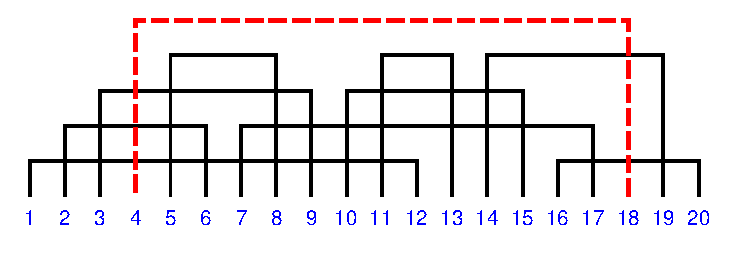
\includegraphics[scale=0.8]{Figs/Probability/ints}
\end{figure}

%ё
\section*{Решения и комментарии}

\subsubsection*{Потерянный посадочный талон}% (THE LOST BOARDING PASS)

Давайте дождёмся когда сотый пассажир поднимется на борт. 
Оставшееся место будет либо то, что указано на его посадочном талоне, либо место первого пассажира.
Все остальные места заняты пассажирами согласно посадочным талонам или теми, что сели первыми.

Так как на каждом шаге ни одному из этих двух мест не было дано никакого предпочтения, вероятность того, что сотый пассажир сядет на своё место равна $50\%$.
\heart

Приведённое здесь рассуждение аналогично тому, что используется, скажем, при подсчёте шансов в Крэпсе (разновиднось игры в кости с двумя кубиками).
После того, как вы выбросили «пойнт»,
(то есть в сумме два кубика дали 4, 5, 6, 8, 9 или 10), вы продолжаете бросать кости до тех пор, пока не выпадет 7 или тот же пойнт.
Чтобы определить вероятность выигрыша (повторный выброс пойнта), вы предполагаете, что следующий бросок последний, и рассчитываете соответственно.
Например, если ваш пойнт --- 5, ваши шансы --- 4 из 10 (потому что имеется 4 способа выбросить 5 и 6 способов выбросить 7).
В случае с потерянным посадочным талоном, один из 99 пассажиров в конце концов сядет на место первого или место сотого, в этот момент оба этих места выбираются с равной вероятностью. 

\medskip

Источник: Дружеские беседы.
В данном случае я услышал эту задачу на конференции «Gathering for Gardner V».
Приведённая здесь версия предоставлена Анде Холройдом. % (Ander Holroyd). %???

\subsubsection*{Все грани кубика}% (ROLLING ALL THE NUMBERS)

Данная классическая задача демонстрирует два важных принципа: среднее время ожидания и линейность математического ожидания. %???
Предположим, вы повторяете эксперимент, вероятность успеха которого равна $p$.
Как долго надо вам ждать успешного исхода? Вы можете вычислить это значение как сумму
\[\sum_{n=1}^\infty n(1-p)^np=1/p,\]
но это не выглядит особо убедительно с интуитивной точки зрения.
Лучше представим, что эксперимент повторяется $n$ раз, и $n$ настолько большое, что доля успешных экспериментов сколь угодно близка к $p$ (закон больших чисел).
Вы можете думать об этих $n$ испытаниях, как об отдельных сериях по $pn$ экспериментов, где каждый эксперимент завершается успехом.
Их средняя длина равна $n/(np)=1/p$.

В задаче требуется выбросить все шесть цифр, и ключевой момент состоит в том, чтобы разбить этот процесс на шесть этапов.
Среднее время, что потребуется для завершения всех этапов, будет тогда равно сумме средних времён каждого этапа.
Теперь, как известно, если проследить за числом различных цифр, которые уже выпали, то первое значение этого числа будет равно 1 (после первого броска) и оно будет, шаг за шагом, увеличиваться на единицу, пока не достигнет 6.
Положим, «этап номер $k$» --- это период, в течении которого уже были выброшены $k-1$ различных цифр, и мы ожидаем появления $k$-той.

Вероятность успеха на этапе номер $k$ равна, всего лишь, числу цифр, ещё не выпавших на кубике, а именно $6-(k-1)$, разделённому на $6$;
значит средняя длина этапа номер $k$ равна $6/(6-k+1)$.
Из этого следует, что среднее время для всего процесса будет
\[\frac66+\frac65+\frac64+\frac63+\frac62+\frac61=14{,}7.\]
\heart

Пожалуй, стоит отметить, что результат был бы совсем другим, если бы мы бросали шесть кубиков одновременно и ожидали, когда выпадут все цифры сразу при одном броске.
Вероятность успеха равна $6{\cdot}5{\cdot}4{\cdot}3{\cdot}2{\cdot}1/6^6$ (смотри, например, последнюю задачу в предыдущей главе), что приблизительно равно $0{,}0154321$.
Следовательно, среднее время ожидания будет состоять из $64{,}8$ попыток, это довольно долго, учитывая, что при одной попытке мы бросаем 6 кубиков одновременно.

\subsubsection*{Нечётная череда решек}% (ODD STREAK OF HEADS)

Данная задача была предложена, но не была использована, на ММО в начале 80-х.%
\footnote{Смотри Murray Klamkin, \emph{International Mathematical Olympiads, 1978--1985} Mathematical Association of America, 1986.}
Она идёт в паре с предыдущей задачей, но здесь надо больше думать.

\medskip

Если мы подсчитаем вероятность того, что мы выбрасываем решку сразу же нечётное число раз, и потом орла, мы получаем 
\begin{align*}\mathbb{P}(\textsc{ро})+ \mathbb{P}(\textsc{ррро})+ \mathbb{P}(\textsc{ррррро})+\dots&=
\\
=(\tfrac12)^2+(\tfrac12)^4+(\tfrac12)^6+\dots&=\tfrac13.
\end{align*}

Если так не удаётся, то есть выпадает орёл (после чётного числа решек), мы должны начинать сначала.
Таким образом, в среднем, нам понадобится три подобных эксперимента.
Но мы хотим посчитать количество бросков, а не экспериментов.

К счастью, мы можем воспользоваться другим свойством математического ожидания:
Если имеется произвольное число $n$ объектов, чья средняя величина равна $s$, тогда средняя общая величина всех объектов равна $s$, помноженному на среднее значение $n$.
Каждый из экспериментов (успешный или нет) заканчивается, когда появляется первый орёл, таким образом, среднее число бросков на эксперимент $1:\tfrac12=2$.
Из этого следует, что
решением задачи будет $2{\cdot}3=6$ бросков.\heart

Есть более красивый способ решения этой задачи.
Пусть ответ равен $x$.
Если мы начинаем с \textsc{о} или \textsc{рр}, то для достижения успеха нам предстоит сделать в среднем ещё $x$ бросков.
Если мы начинаем с \textsc{ро}, то это уже успех.
Отсюда
\[x=\tfrac12 \cdot(1+x)+\tfrac14 \cdot(2+x)+\tfrac14 \cdot2.\]
Что нам даёт $x=6$.

\subsubsection*{Три кубика}% (THREE DICE)

Вообще-то, эта игра предлагаются в некоторых казино, в Америке она называется чак-э-лак или бёрд кейдж%
\footnote{англ. Bird Cage --- \emph{птичья клетка}; кубики в этой игре обычно бросаются в клетке}. %???
Справедливо заявить, что уже один этот факт сам по себе является доказательством без вычислений того, что игра идёт в пользу казино.

Однако есть довольно красивый математический способ показать это, и он применим также и к другим азартным играм.
Представим себе, что у нас шесть игроков, все ставят по 1 доллару на разные числа, и затем бросаются кубики.
Казино никогда не проигрывает!
Если выпадают три различных числа, крупье забирает 3 доллара у проигравших и отдаёт их выигравшим.
В остальных случаях крупье забирает 4 или 5 долларов, отдавая выигравшим только 3.\heart

Итак, игра идёт в пользу казино, если игроки делают ставки подобным образом.
Но, значит ли это, что она \emph{всегда} в пользу казино?
Да, значит --- статистически, казино выигрывает или проигрывает не независимо от того, кто как и сколько ставит.

Конечно, совсем несложно определить напрямую, что чак-э-лак --- дело проигрышное.
Вероятность того, что выпадут три разных числа равна $6{\cdot}5{\cdot}4/6^3=5/9$.
Игрок, делающий ставку, рискует уже здесь, так как вероятность того, что его число одно из выпавших, равна $1/2$.
С вероятностью $1/36$ на всех кубиках выпадет одно и тоже число;
и тут игрок получает $3$ доллара с вероятностью $1/6$ и теряет 1 доллар всё остальное время, средний проигрыш будет $1/3$ доллара.
И, наконец, оставшиеся $5/12$ времени игрок выигрывает $2$ доллара с вероятностью $1/6$, и теряет $1$ доллар с вероятностью $2/3$, в среднем он проигрывает $1/6$ доллара.
В общем, его потери составят $1/36{\cdot}1/3 + 5/12{\cdot}1/6 = 17/216$; то есть, примерно, $8$ центов с доллара.

\medskip

Игру можно сделать честной, давая игроку 3 доллара вместо 2 при выпадении двух одинаковых чисел 
и 5 долларов вместо 3, когда выпадают 3 одинаковых числа.

\medskip

Эта задача впервые появилась в «Энциклопедии головоломок» Сэма Лойда, под редакцией Сэма Лойда II, 1914\footnote{\emph{Sam Loyd’s Cyclopedia of 5000 Puzzles, Tricks, and Conundrums,} edited by Sam Loyd II, 1914}.
Сэм Лойд (старший), 1841---1911, хорошо известен многим читателям как непревзойдённый мастер занимательных задач и величайший американский головоломщик.

\subsubsection*{Намагниченные доллары}% (MAGNETIC DOLLARS)

Большинство людей предположат, что урна с меньшим количеством сюзанн практически ничего не стоит.
И действительно, недавно сидя в ресторане с профессиональными математиками, в ответ на данный вопрос только один был готов предложить 100 долларов, остальные же давали не больше 10.

На самом деле, эта урна стоит, в среднем, хорошую четверть миллиона долларов.
Вероятность распределения конечного содержимого для двух урн однородна.
Вероятность того, что, скажем, в первой урне в конце окажется только одна сюзанна такая же, как и вероятность того, что там будет 451 382 сюзанны.

Это легко доказывается по индукции, но я считаю гораздо интереснее приведённую ниже аналогию с тасованием карт.
Представим себе колоду из 999 999 карт, из которых только одна --- красная.
Перетасуем их очень хорошо следующим способом.
Положим красную карту на стол.
Теперь берём вторую карту (любую) и кладём её с одинаковой вероятностью на или под красную карту.
Есть три варианта, куда можно поместить следующую карту, с одинаковой вероятностью выбираем один из них и вставляем карту.
Когда последняя карта добавлена, на столе у нас --- идеально перетасованная колода карт.

Но заметьте: когда сверху красной карты находятся $x-1$ карта, а снизу $y-1$, то вероятность того, что следующая карта окажется над красной равна $x/(x+y)$.
Таким образом, карты сверху красной карты ведут себя также, как сюзанны (не считая начальной) из первой урны, а карты снизу --- как из второй.

Из того, что в конечной колоде красная карта может с равной вероятностью оказаться на любой высоте, следует однородность распределения для сюзанн.\heart
 
Задачу (парадокс?) о намагниченных долларах иногда называют «Урной Пойа»,\footnote{Смотри N. Johnson and S. Kotz, \emph{Urn Models and Their Applications: An Approach to Modern Discrete Probability Theory,} Wiley, New York, 1977.} по имени великого математика, популяризатора науки и любителя головоломок Дьёрдя П\'{о}йа, 1887---1985.
Нетрудно показать, что если подбрасывается бесконечное количество сюзанн, то в пределе с вероятностью, равной 1, процент сюзанн, попавших в первую урну, задаётся однородным распределением на единичном интервале.

\subsubsection*{Торговля вслепую}% (BIDDING IN THE DARK)

Вы не должны делать предложение.
Если вы предложите $x$ долларов, то ожидаемая стоимость приборчика для хозяина, при условии, что \emph{он его продаёт}, будет равна $x/2$ доллара.
Следовательно, для вас ожидаемая стоимость приборчика, если вы его получите, будет равна $1{,}8 {\cdot} x/2=0{,}9{\cdot}x$ долларов.
Таким образом, в среднем, вы теряете деньги, если покупаете приборчик и, конечно же, ничего не теряете и не выигрывайте, если не покупаете.
Так что глупо предлагать.\heart

Источник: Майя Бар Хиллел, университет в Иерусалиме.

\subsubsection*{Случайные интервалы}% (RANDOM INTERVALS)

У этой задачи любопытная история.
Моему коллеге (Эду Шнайнерману из университета Джона Хопкинса) и мне нужно было решить эту задачу, чтобы вычислить диаметр так называемого \emph{случайного интервального графа}. 
Вначале мы доказали, что асимптотическое значение этой вероятности равно $2/3$.
Потом, много и беспорядочно интегрируя, нашли, что вероятность того, что найдётся интервал, который пересекает все остальные \emph{в точности} равна $2/3$ (для любого числа интервалов начиная с двух).

Джойс Джастич, %(Joyce Justicz)
будучи в то время моим аспирантом в университете Эмори, придумал следующее комбинаторное доказательство.

Предположим, конечные точки интервалов выбираются из множества $\{1,2,\dots,2n\}$.
Обозначим $2n-4$ из их концов символами $A(1)$, $B(1)$, $A(2)$, $B(2),\dots, A(n-2)$, $B(n-2)$ согласно следующему рекурсивному правилу.
Будем говорить что точки $\{n+1, \dots , 2n\}$ лежат с правой стороны, а точки $\{1, \dots , n\}$ --- с левой.
Положим $A(1)=n$ и $B(1)$ --- парная ей точка.
Допустим, мы уже выбрали точки до $A(j)$ и $B(j)$. 
Если $B(j)$ лежит с левой стороны, тогда $A(j+1)$ выбирается самой левой из невыбранных ещё точек правой стороны, и $B(j+1)$ --- её пара.
Если $B(j)$ лежит с правой стороны, тогда $A(j+1)$ выбирается самой правой из необозначенных ещё точек левой стороны, и снова $B(j+1)$ --- её пара.

Если $A(j) < B(j)$, мы говорим, что интервал «ушёл направо», в обратном случае --- он «ушёл налево».
Точки, обозначенные $A({\cdot})$ будем называть внутренними концами интервала, остальные --- внешними.

\begin{figure}[h!]
\centering
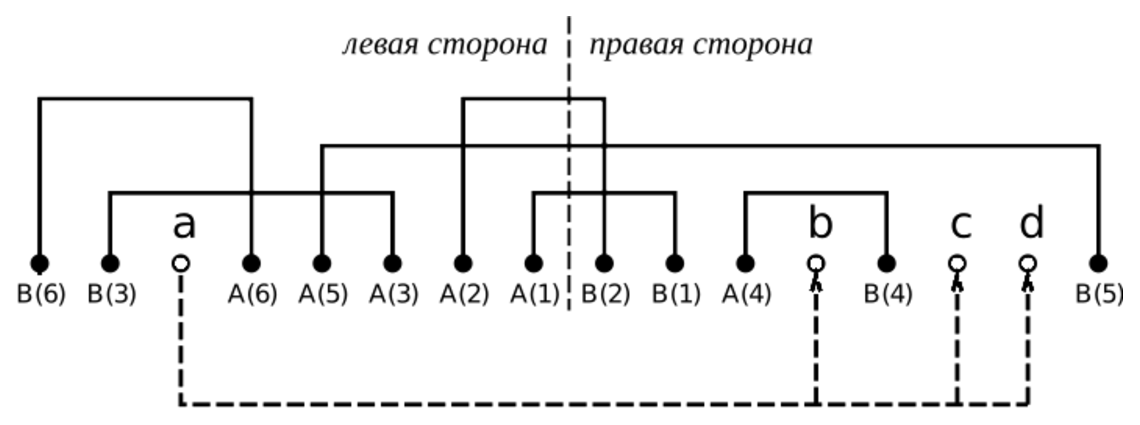
\includegraphics[scale=0.55]{Figs/Probability/labeling-ru}
\end{figure} 

Используя индукцию по $j$, легко доказать, что после того, как выбраны $A(j)$ и $B(j)$, либо одинаковое количество точек было выбрано на каждой из сторон (в случае если $A(j) < B(j)$), либо на левой стороне было выбрано на две точки больше (в случае если $A(j) > B(j)$).

После того, как мы обозначили точки $A(n-2)$ и $B(n-2)$, остаётся четыре необозначенных точки концов интервалов, назовём их $a<b<c< d$.
Мы утверждаем, что из трёх равновероятных способов разбиения этих точек на пары, два приведут к «больш\'{о}му» интервалу, пересекающему все остальные, а один способ --- нет.

В случае если $A(n-2) < B(n-2)$, точки $a$ и $b$ находятся слева, а $c$ и $d$ --- справа;
в противном случае только $a$ находится слева.
В любом случае, все внутренние концы интервалов лежат между точками $a$ и $c$, иначе одна из них была бы выбрана.
Из этого следует, что интервал $[a,c]$ пересекает все остальные, и точно также $[a,d]$.
То есть, если $a$ не в паре с $b$, то у нас большой интервал.

Допустим, напротив, что наши пары именно $[a, b]$ и $[c, d]$.
Ни одна из них не может быть большим интервалом, так как они не пересекаются с друг другом.
Предположим теперь, что существует другой большой интервал, скажем $[e,f]$ с концами $A(j)$ и $B(j)$.

Если точки $a$ и $b$ находятся слева, внутренние концы $A(j)$ лежат между $b$ и $c$, таким образом $[e, f]$ не может пересекать оба интервала $[a, b]$ и $[c, d]$, что противоречит нашему предположению.

В оставшемся случае, так как $[e, f]$ пересекает $[c, d]$, $f$ является внешним концом интервала. 
В этом случае $f=B(j)$, то есть отрезок $[e, f]$ ушёл направо.
Поскольку последняя выбранная пара точек ушла налево, существует $k>j$, для которого $A(k)>B(k)$ и $A(k-1)<B(k-1)$.
В этом случае $A(k)$ лежит слева и значит $A(k) < A(j)$, так как $A(k)$ --- левосторонняя внутренняя точка, выбранная позже.
Тогда $[A(j), B(j)]$ не пересекает $[B(k), A(k)]$; это последнее противоречие доказывает наше утверждение.
\heart

Используя данное рассуждение с чуть большей аккуратностью, можно доказать, что 
для $k < n$ , вероятность того, что в семействе случайных $n$ интервалов найдётся, по меньшей мере, $k$ интервалов, которые пересекают все остальные, равна
\[\frac{2^k}{\binom{2k+1} k}\]
и она не зависит от $n$.
Здесь $\binom n k$ означает \emph{биноминальный коэффициент}, то есть число подмножеств размера $k$ из множества размера $n$, и он равен $n(n-1)(n-2)\cdots(n-k+1) /(k(k-1)(k-2)\cdots1)$.

\chapter*{География(!)}
\addcontentsline{toc}{chapter}{География(!)}

\setlength{\epigraphwidth}{.45\textwidth}
\epigraph{Без географии мы были бы нигде.}{---Джимми Баффет (1946---)}%???- или --- 

Да, данная глава не принадлежит этой книге. %(не из этой книги).
Некоторые из задач, представленных здесь, конечно, математические по своей природе, %(mathematical in nature) 
но, в основном, они включены в книгу потому, что доставляют, как мне кажется, большое удовольствие любителям математических головоломок.
Мой издатель уверял меня, что без «Географии» стоимость книги была бы такой же.

Так что эта глава как бы бесплатное приложение, и её можно пропустить с чистой совестью.

Основная тема приведённых ниже задач --- поверхность планеты Земля.
Хотя предпочтение всё-таки отдаётся моей родине --- Соединённым Штатам Америки. 
О чём прошу прощения у читателей из других стран.
Я буду очень благодарен за подобные задачи про разные страны, присланные мне на pw@akpeters.com.

Несколько из этих задач показывают до какой степени %( test the degree) 
картографическая проекция %( на плоскость) (planar projections) 
искажает наше представление о земном шаре. %(глобусе, globe).
Вот одна из них: 

\subsection*{Африка}
\rindex{Африка}

Какой штат США ближе всего к Африке? 

\paragraph{Решение:} Штат Мэн.\heart
  
Он совсем не близко --- проверьте по глобусу.
Но если вы летите по ортодромии (в картографии и навигации ортодромия --- название кратчайшего расстояния между двумя точками на поверхности Земли) из Майами, скажем, в Касабланку, вначале ваш курс %(путь)
будет лежать на Северо-Восток вдоль восточного побережья и пройдёт очень близко к штату Мэн.
%(not missing Maine by much)

\medskip

Дальше попробуйте сами.

\subsection*{На восток от Рино}%EAST OF RENO 
\rindex{На восток от Рино}

Какой самый большой город в США к востоку от Рино, Невада и к западу от Денвера, Колорадо? 

\subsection*{Телефонный звонок}%(THE PHONE CALL) 
\rindex{Телефонный звонок}

Представьте, что вы звоните из какого-то штата Восточного побережья в один из штатов Западного побережья США, и на обеих концах одно и то же время суток.
Как такое может быть? 
  

\subsection*{Диаметр Соединённых штатов}%(THE DIAMETR OF US)  
\rindex{Диаметр Соединённых штатов}

В каких двух штатах находятся две самые удалённые точки США? 
  

\subsection*{На юг от Ки-Уэст}% ( SOUTH FROM KEY-WEST) 
\rindex{На юг от Ки-Уэст}

Если вы летите на юг от города Ки-Уэст, Флорида, какая южно-американская страна вам 
встретится первой? 

\subsection*{Индейцы на среднем западе}% (INDIANS IN THE MIDWEST) 
\rindex{Индейцы на среднем западе}

Среди штатов Среднего Запада США только один имеет название не индейского происхождения? Который?    

\subsection*{Самый большой второй по величине город}% (THE LARGEST SECOND-LARGEST CITY)  
\rindex{Самый большой второй по величине город}

Какой город в США самый большой среди городов с одинаковыми именами, но не больше города США с таким же именем?

\medskip

Эта формулировка может показаться несколько путаной.
Спросим по-другому: скажем, что город (в США) «находится в тени», если существует б\'{о}льший город с таким же именем.
Например, Портланд, штат Мэн, находится в тени города Портланд, штат Орегон.

Итак, наш вопрос прозвучит теперь так: какой наибольший город в США находится в тени?   

\subsection*{Естественные границы}% (THE NATURAL BORDERS) 
\rindex{Естественные границы}

Граница штата может быть естественной (определяться водоёмами, горами и пр.) или 
закреплённой в законе искусственной линией --- в одном знаменитом случае (связанном со штатом Делавэр и Пенсильванией ) --- это дуга окружности.
Три штата --- Колорадо, Юта и Вайоминг имеют только искусственные границы.
Какой штат обладает только естественными границами?   

\subsection*{Непересекаемые границы}% (THE UNCROSSABLE BORDER) 
\rindex{Непересекаемые границы}

Говоря о границах штатов, можете ли вы найти такой штат, который нельзя пересечь на автомобиле? Другими словами укажите два штата, имеющих общую границу, через которую, однако, невозможно напрямую проехать на автомобиле из одного штата в другой?   

\subsection*{Отдел странных названий}% (DEPARTMENT OF ODD NAMES) 
\rindex{Отдел странных названий}

Что особенного в неком местечке, именуемом Уэст-Куодди-Хед, %(West Quoddy Head) 
штат Мэн?   

\subsection*{Городской и деревенский}%(URBAN AND RURAL) 
\rindex{Городской и деревенский}

Данная задача скорее более социологического плана.
В наши дни большинство американцев --- порядка 75\% --- живут в так называемых «городских агломерациях (урбанизированных зонах)».
Перепись населения 2000 года относит к «городскому» 100\% населения одного из штатов и только 27,6\% населения другого штата, который отдалён от первого всего лишь на несколько сот миль.
Можете назвать эти два штата?   

\subsection*{Города на север и на юг}% (CITIES NORTH AND SOUTH) 
\rindex{Города на север и на юг}

Как обстоит дело с вашей визуализацией континентов?
Проверьте, как точно вы представляете себе %(визуаилизируете) 
карту мира.
Расставьте следующие четыре города по порядку с юга на север: 
Галифакс, Новая Шотландия; %(Halifax, Nova Scotia) 
Токио, Япония; %(Tokyo, Japan); 
Венеция, Италия; %(Venice, Italy); 
Алжир, Алжир. %(Algiers, Algeria).

\subsection*{Город в один слог}% (THE ONE-SYLLABLE CITY) 
\rindex{Город в один слог}

Какой город в США, имя которого состоит из одного слога, самый большой? 

\subsection*{Вашингтоны и феминисты}%(WASHINGTONS AND FEMINISTS) 
\rindex{Вашингтоны и феминисты}

Данная задача --- это своеобразный тест на знание не только карты штатов США, но и их английских названий.
Чтобы найти решение этой задачи, вам придётся пользоваться исключительно оригинальными английскими названиями штатов.
Итак, вопрос: 

Сможете ли вы проложить маршрут для автомобиля из города Сиэтл, штат Вашингтон, 
 в Вашингтон, округ Колумбия, таким образом, чтобы названия всех штатов, через которые вы планируете проехать, начинались только с букв, составляющих слово «WOMAN»?
%???добавленно 

\medskip

Наша последняя географическая задача напоминает нам, что пора возвращаться к математике. %(signals us a(slight) return to mathematics) направляет 

\subsection*{Учёный и медведь}%(THE NATURALIST AND THE BEAR) 
\rindex{Учёный и медведь}

Учёная-биолог покинула лагерь экспедиции, прошла 10 миль на юг, затем 10 миль на восток и тут заметила и сфотографировала медведя.
Пройдя 10 миль на север, она пришла обратно в лагерь.

\medskip

Вы не видели фотографии, но всё равно знаете, какого цвета был медведь, не так ли?

%ё
\section*{Решения и комментарии}

Для проверки правильности ответов бы можете воспользоваться атласом, глобусом, альманахом или итогами переписи населения США 2000 года. 
Давайте посмотрим, насколько верны были ваши предположения...
%(догадки)

\subsubsection*{На восток от Рино}% (EAST OF RENO)

Вопрос о самом большом городе может оказаться довольно щекотливым; 
%(awkward question) 
стандартно это понятие определяется количеством населения (не площадью!) в официальных границах города, что, безусловно, может привести к неверным выводам
при наличии городских агломераций.
%(урбанизированных зон)
%(can be misleading with respect to metropolitan area).
Так, например, согласно данным альманаха город Джэксонвилл, штат Флорида, представляется больше, чем Атланта, штат Джорджия, несмотря на то, что население всей городской агломерации Атланты превышает население Джэксонвилла почти в четыре раза.

\medskip

Но в нашей задаче нам не понадобятся такие тонкости. Самый большой город к востоку от Рино и к западу от Денвера, в любом случае, Лос-Анджелес, Калифорния.                                 \heart

\subsubsection*{Телефонный звонок}%ТЕЛЕФОННЫЙ ЗВОНОК (THE PHONE CALL)

«Восточное побережье» Соединённых Штатов Америки включает в себя восточные штаты, имеющие выход к Атлантическому океану, от штата Мэн на севере до штата Флорида на юге. 
К «Западному побережью» относятся штаты Вашингтон, Орегон и Калифорния,
к которым, если хотите, вы можете добавить Аляску и даже Гавайи, но это не так уж важно в данном случае. %(but it doesn’t help).

Обычно, делая подобные звонки, мы имеем разницу во времени между Восточным и Западным побережьем в 3 часа. Мы можем избавиться от одного часа, позвонив из западного района так называемой «ручки ковша» Флориды --- её северо-западной части, % ( Florida panhandle) 
скажем, из города Пенс\'{а}кола, который находится в Центральном часовом поясе. 
Чтобы избавиться ещё от одного часа, мы звоним в один из городов самого восточного района штата Орегон (скажем, Онтарио), в котором Горное время. 

Оставшийся час исчезнет, если звонок будет сделан из Пенсаколы между двумя и тремя часами ночи, при переходе с Летнего времени на Зимнее. 
В этот момент в Центральном часовом поясе время уже переведут на один час назад, а Горное время всё ещё будет прежним.\heart 

       
                                  
\subsubsection*{Диаметр Соединённых штатов}%ДИАМЕТР СОЕДИНЁННЫХ ШТАТОВ (THE DIAMETR OF US) 

Очевидно, это либо Гавайи и Мэн, либо Аляска и Флорида. Или это Гавайи и Аляска?

\medskip

Удивительным образом, ни одно, ни другое, ни третье. Правильный ответ --- Гавайи и Флорида.\heart

\subsubsection*{На юг от Ки-Уэст}%НА ЮГ ОТ КИ-УЭСТ ( SOUTH FROM KEY-WEST)

Это, без сомнения, каверзный вопрос. %(a trick question). 
Вы не пересечёте ни одну страну Южной Америки. 
Ваш путь пройдёт к западу от континента. 
%(Ваш путь пройдёт вдоль западного побережья всего континента.)
\heart

\subsubsection*{Индейцы на среднем западе}%ИНДЕЙЦЫ НА СРЕДНЕМ ЗАПАДЕ (INDIANS IN THE MIDWEST)

По определению к штатам Среднего Запада относятся Миннесота, Висконсин, Айова,
Иллинойс, Миссури, Мичиган, Огайо, Канзас и Небраска --- все названия индейского
происхождения, и остаётся ответ --- Индиана!\heart

Любопытно, что только один штат к востоку от Миссисипи имеет столицу, чьё имя индейского происхождения --- Флорида (Таллахасси).

\subsubsection*{Самый большой второй по величине город}%САМЫЙ БОЛЬШОЙ ВТОРОЙ ПО ВЕЛИЧИНЕ ГОРОД (THE LARGEST SECOND-LARGEST CITY)  

Портланд, штат Мэн? Спрингфилд, Где-нибудь? 
Частые, но не верные предположения.
До 1975 года или около того, правильный ответ был бы Канзас-Сити, штат Канзас, который затеняется городом Канзас-Сити, Миссури.
Затем некоторое время победителем был Колумбус, Джорджия, находящийся в тени столицы Огайо. Однако, мы живём в эпоху пригородов, %(in the age of suburbia), 
перепись населения 2000 года показывает, что теперь городу Глендейл, штат Калифорния (находится в тени Глендейла, Аризона) принадлежит эта сомнительная %(obscure) 
честь.\heart

\subsubsection*{Естественные границы}%ЕСТЕСТВЕННЫЕ ГРАНИЦЫ (THE NATURAL BORDERS)

Конечно, Гавайи имеют только естественные границы. Возможно, вы подумали, что это было слишком легко, но люди часто не видят, что находится у них под носом. 
%(не замечают очевидного) %(folks often have a blind spot).
\heart

\subsubsection*{Непересекаемые границы}%НЕПЕРЕСЕКАЕМЫЕ ГРАНИЦЫ (THE UNCROSSABLE BORDER)

Здесь намного сложнее. Висконсин и Мичиган имеют общую длинную границу по озеру Мичиган, но вы можете пересечь её на пароме Манитовок-Ладингтон, сидя в своей машине. Паром из Монток Пойнт %(Mantauk Point) 
(штат Нью-Йорк) на остров Блок %(Block Island) 
(штат Род-Айленд) пересекает не очень хорошо известную границу между этими двумя штатами, и он только для пассажиров. 
Возможно, существуют и другие решения данной задачи.\heart
                             

Можно задать схожий вопрос о части штата, попасть в которую на автомобиле из остального штата возможно только, проехав через другой штат (или Канаду, в случае с 
Пойнт Робертс). %(Point Roberts). 
Существует несколько таких мест, особенно около вечно меняющейся реки Миссисипи.

\subsubsection*{Отдел странных названий}%ОТДЕЛ СТРАННЫХ НАЗВАНИЙ (DEPARTMENT OF ODD NAMES)

Уэст-Куодди-Хед %(West Quoddy Head) 
--- самая восточная точка континентальных штатов США.\heart
                            

Иногда вам может встретиться утверждение, что, если опустить требование «континентальный», мыс Врангеля %(Cape Wrangel) 
на острове Атту, %(Attu Island) 
штат Аляска, является самой восточной точкой США, но я не принимаю в рассчёт эти «Гринвич-централизованные» доводы. 
%(but I do not buy Greenwich-centered reasoning) 
Назовёте ли вы мыс Врангеля самой восточной точкой Аляски?

\subsubsection*{Городской и деревенский}%ГОРОДСКОЙ И ДЕРЕВЕНСКИЙ (URBAN AND RURAL)

Нью-Джерси и Вермонт. Эту и множество другой интересной информации вы можете найти на сайте:\\
\texttt{http//www.census.gov/prod/2002pubs/01statab/pop.pdf} 
 \heart                          

\subsubsection*{Города на север и на юг}%ГОРОДА НА СЕВЕР И НА ЮГ (CITIES NORTH AND SOUTH)

Токио, Алжир, Галифакс и, наконец, Венеция. Широты, соответственно
$35^\circ 40’$ с.ш.; $36^\circ 50’$ с.ш.; $44^\circ 53’$ с.ш.; и $45^\circ 26’$ с.ш. 
Обратите внимание --- последние два города разделяет 45-я параллель, и это позволяет нам яснее увидеть, что Венеция находится севернее. Один уроженец Новой Шотландии однажды проспорил мне по этому случаю 1 доллар.%по этому случаю???
\heart

\subsubsection*{Город в один слог}%ГОРОД В ОДИН СЛОГ (THE ONE-SYLLABLE CITY)

Йорк, штат Пенсильвания, и Трой, штат Нью-Йорк, называются чаще всего, но всё же Флинт, штат Мичиган, несмотря на существенное сокращение населения за последние годы, остаётся единственным однослоговым городом в США с населением более 100 тысяч человек.
Хотя, если судить по тому, как произносят названия городов местные жители, победителем, несомненно, будет Нью-Арк («Норк», с длинным «о»), штат Нью-Джерси. \heart

\subsubsection*{Вашингтоны и феминисты} %ВАШИНГТОНЫ И ФЕМИНИСТЫ (WASHINGTONS AND FEMINISTS)

Без проблем. Вначале ваш маршрут пойдёт на юг --- через Орегон (Oregon), 
Неваду (Nevada) 
и Аризону, (Arizona), 
затем на восток сквозь Нью-Мексико (New Mexico) 
в Оклахомовскую «ручку ковша», из северо-восточного угла Оклахомы (Oklahoma) 
вы попадаете в Миссури (Missouri). 
Здесь вам надо будет повернуть на север и из северо-западного угла штата проехать в Небраску (Nebraska), продолжая путь на запад в Вайоминг (Wyoming) и на север в Монтану (Montana) --- довольно большой круг для того, чтобы объехать Айдахо (Idaho). 
В конце концов, вы сможете снова развернуться и поехать на восток через Северную Дакоту (North Dakota), 
Миннесоту (Minnesota), 
Висконсин (Wiskonsin) 
и Мичиган (Michigan).
Теперь берите курс на юг в Огайо (Ohio) и на восток сквозь Западную Виргинию (West Virginia) в Мериленд (Maryland),
 и в Вашингтон (Washington DC), округ Колумбия.\heart

Чтобы пройти по этому маршруту, вам придётся несколько раз %(или на долгое время) 
покинуть национальную систему межштатных автомагистралей, но мы предполагаем, вы никуда не торопитесь.

\subsubsection*{Учёный и медведь}%УЧЕНЫЙ И МЕДВЕДЬ (THE NATURALIST AND THE BEAR)

Начальная идея была, конечно, что лагерь экспедиции находился на Северном полюсе, так как маршрут учёной (10 миль на юг, 10 миль на восток и 10 миль на север) является замкнутым контуром, %(to have been a closed loop), 
следовательно медведь был белый.

Однако, как было замечено в одной из рубрик %(колонок) 
Мартина Гарднера, %(Martin Gardner’s columns), 
на поверхности Земли существует бесконечно много других точек, где подобный путь будет замкнутым.

Некоторые из этих точек лежат на окружности с центром в Южном полюсе и радиусом немного меньше $10 + \tfrac5\pi$ миль.
Начав прогулку с такой точки, наша учёная после первых 10 миль окажется в некой точке $P$, 
находящейся на расстоянии чуть меньше $\tfrac5\pi$ миль от Южного полюса. 
Повернув на Восток и пройдя 10 миль, она обогнёт весь мир и вернётся в точку $P$, откуда 10 миль на Север приведут её обратно в лагерь.

Другая окружность, радиусом чуть меньше $10 + \tfrac5{2\pi}$ миль тоже сработает, во второй (Восточной) части пути наша учёная должна будет 2 раза обойти вокруг Южного полюса и так далее.

В Антарктике медведи не водятся, но если бы водились, то, наверное, были бы белыми.
Так что ответ задачи не изменится.\heart

\end{document}
%ссылки  на источник даются в разном формате, я бы его униформуизировал 
%проверь разбивку на абзацы, иногда она у тебя не та, что у винклера 
%вы или Вы везде одинакого
%\heart после формул
%т.е. --> т.~е.
%кавычки «», ", выделения...
